\documentclass[11pt,onecolumn]{article}

% ── Packages ──────────────────────────────────────────────────────────────────
\usepackage[margin=1in]{geometry}
\usepackage{amsmath,amssymb}
\usepackage{graphicx}
\usepackage{booktabs}
\usepackage{hyperref}
\usepackage{natbib}
\usepackage{microtype}
\usepackage{xcolor}
\usepackage{lineno}
\usepackage{setspace}
\usepackage{caption}
\usepackage{subcaption}
\usepackage{authblk}
\usepackage{array}
\usepackage{tabularx}
\usepackage{orcidlink}

\hypersetup{
  colorlinks=true,
  linkcolor=blue!60!black,
  citecolor=blue!60!black,
  urlcolor=blue!60!black,
}

\doublespacing
\linenumbers

% ── Title block ───────────────────────────────────────────────────────────────
\title{\textbf{Mouse V1 Passes Through a Transient Low-Dimensional State
of Peak Cross-Individual Representational Consistency During Natural
Image Viewing}}

\author[1]{Z. Jana\orcidlink{0009-0009-3316-7476}}
\affil[1]{Department of Computer Science and Engineering,
The American University in Cairo}

\date{}

% ──────────────────────────────────────────────────────────────────────────────
\begin{document}
\maketitle

% ── Abstract ──────────────────────────────────────────────────────────────────
\begin{abstract}

When different mice view the same natural image, their primary visual cortex (V1) populations share a measurable fraction of representational structure, yet whether this cross-individual agreement is constant across the visual response or concentrated in a particular moment is unknown. Using millisecond-resolution representational similarity analysis (RSA) of Neuropixels recordings from all 32 \texttt{brain\_observatory\_1.1} sessions of the Allen Brain Observatory (32 mice, 118 natural images), we show that cross-mouse consistency is dynamic: it rises to a transient peak $\sim$100~ms after stimulus onset (Spearman $r = 0.307$) before decaying to a lower sustained floor ($r = 0.182$). This peak coincides precisely with a several-fold collapse in the effective dimensionality of the shared representation, and dimensionality and consistency remain tightly coupled across the entire post-stimulus epoch ($r = -0.929$ on independent, non-overlapping windows). The moment mice agree most is the moment the population code is most compressed. This transient state is specific to naturalistic stimuli --- static gratings produce a flat curve with no transient peak --- and is highest in V1, lower across extrastriate cortex, and substantially weaker in thalamus.

To probe what produces this compression, we dissociated fast-spiking (FSU, putative inhibitory) from regular-spiking (RSU) units. Individual FSU units carry $\sim$1.9$\times$ the cross-mouse-consistent signal of RSU units (Mann--Whitney $p = 1.4 \times 10^{-45}$), an advantage that survives controlling for firing magnitude and sparsity and that includes a sharper transient shape; optotagged PV$^+$ interneurons behave consistently with this dissociation. A minimal mechanistic model — each unit's early response shrunk toward the population mean in proportion to measured FSU population activity — reproduces the timing of this collapse and recovery (cross-validated shape-$R^2 = 0.81$ across held-out sessions) but systematically underestimates its magnitude, indicating FSU-gated shrinkage contributes to, but does not fully account for, the observed compression. Together, these results show that mouse V1 passes through a transient, low-dimensional state during natural image viewing --- plausibly imposed by fast-spiking inhibition --- and that this state is precisely when representational structure is most shared across individuals.

\end{abstract}

\noindent\textbf{Keywords:} primary visual cortex; representational
similarity analysis; cross-individual variability; fast-spiking
interneurons; participation ratio; neural geometry; Allen Brain
Observatory

\newpage

% ── Introduction ──────────────────────────────────────────────────────────────
\section{Introduction}

A central goal of systems neuroscience is to identify which features of
neural population activity are canonical --- shared across individuals of
the same species exposed to the same stimuli --- and which are
idiosyncratic, reflecting individual developmental history, anatomy, or
ongoing internal state. In primary visual cortex, population responses
to natural images vary substantially across individuals in absolute firing
rates and in which neurons are active, yet downstream circuits must extract
a stable visual representation regardless. One quantitative handle on this
problem is cross-individual representational consistency: the degree to
which different animals agree on the relational structure of their
population responses --- which stimuli are represented as similar to which
others --- even when their absolute responses differ
\citep{kriegeskorte2008}. High cross-individual consistency implies that a
canonical representational geometry is expressed in V1, potentially
reflecting shared tuning properties that emerge from common developmental
programs and anatomical connectivity.

The geometry of V1 population representations has been characterised in
terms of dimensionality \citep{stringer2019}, cross-animal manifold
alignment \citep{williams2021}, and the degree to which response structure
is predicted by deep convolutional neural network (CNN) features
\citep{yamins2016,cadena2019}. These studies have generally treated
representational consistency as a static quantity, computed over a broad
temporal window that collapses the entire visual response into a single
point estimate. However, visual responses in V1 are dynamically structured:
an early feedforward volley arriving at approximately 40--45~ms post-onset
is followed by recurrent and feedback contributions that emerge around
80~ms and later \citep{lamme2000,kirchberger2023}. Whether cross-individual
agreement on representational structure is uniformly distributed across
this epoch, or concentrated in a particular temporal component reflecting
a specific circuit mechanism, is unknown.

Here we ask whether the V1 population code passes through a transient,
low-dimensional regime during the visual response, and if so, whether that
is the moment at which different animals' representations are most alike.
A code transiently compressed into a small number of stereotyped dimensions
is, almost by construction, more likely to look similar across individuals
than a code spread across many idiosyncratic dimensions. Cross-individual
RSA consistency is therefore not only a measure of agreement in its own
right, but a sensitive, model-free readout of when the population code is
in such a compressed, canonical state.

Having established whether and when such a state occurs, we then ask what
produces it. Fast-spiking interneurons --- the dominant subtype of which
expresses parvalbumin (PV$^+$) --- are a strong mechanistic candidate.
Putative fast-spiking interneurons in V1 receive strong thalamic drive and
fire with short latency and high spike-timing precision
\citep{zhuang2013,bereshpolova2020}, properties consistent with a role for
PV$^+$ cells specifically, which receive intense monosynaptic
thalamocortical drive \citep{cruikshank2007}, have directly characterised
visual response properties in genetically identified mouse V1 recordings
\citep{runyan2010}, and provide powerful lateral inhibition onto pyramidal
cells through perisomatic synapses \citep{freund2007}. The classical
iceberg effect posits that inhibition sculpts a broad excitatory input into
a sharper, more selective response \citep{shapiro2022, troyer1998}. If
this inhibitory sharpening operates at the population level, fast-spiking
units should show a sharper version of any transient compression than
broad-spiking units, and a model in which FSU activity gates shrinkage of
the population toward a common response profile should reproduce the
timing of the observed dimensionality collapse.

We test these two questions in sequence using the Allen Brain Observatory
Visual Coding Neuropixels dataset \citep{siegle2021}, which provides
simultaneous recordings from hundreds of V1 units across 32 mice viewing an
identical set of 118 natural images. We first apply a sliding-window RSA
approach at 10~ms temporal resolution to characterise the full temporal
trajectory of cross-individual consistency, and pair it with participation
ratio analysis to test directly whether peak consistency coincides with
minimum dimensionality. We then turn to mechanism: waveform-based
cell-class dissociation, optotagged PV$^+$ recordings, and a cross-validated
model testing whether FSU population activity, acting as a gating signal
for shrinkage toward the population mean, can reproduce the
participation-ratio trajectory itself. As mechanistic contrasts, we compare the temporal profiles
of natural scenes with static gratings and examine how consistency varies
across cortex, thalamus, and a hippocampal control region. Extended predictor, robustness, and validation
analyses that support but do not change these headline results are
reported in the Supplementary Information.

% ── Results ───────────────────────────────────────────────────────────────────
\section{Results}

\subsection{Cross-mouse consistency in V1 is substantial and shaped by
image sparsity}

We used recorded spike times from VISp units in 32 mice viewing 118 natural
images (250~ms each, 50 repetitions per image) from the Allen Brain
Observatory \textit{brain\_observatory\_1.1} dataset \citep{siegle2021}, see Methods \ref{Methods:Dataset}.
For each session, units passing quality control ($n = 14$--$110$ units per
session) \ref{Methods:QC} were used to construct a $118 \times n_\mathrm{units}$
trial-averaged, column-wise z-scored response matrix, and cross-mouse
consistency was quantified for each image as the mean Spearman rank
correlation, across all $\binom{32}{2} = 496$ mouse pairs, of that image's
cosine-similarity profile to the other 117 images, see Methods \ref{Methods:RSA}.

Within-mouse response-vector reliability was near unity (mean $r = 0.978$,
range $[0.968, 0.983]$), confirming the analysis is not limited by
within-session trial noise; the more directly comparable reliability
estimate --- computed in the same image-by-image similarity space (RDM
space) that consistency itself is computed in --- was lower but still high
(mean $r = 0.832$, range $[0.609, 0.929]$), see Methods \ref{Methods:Within-mouse reliability}. Against this ceiling,
cross-mouse consistency was significant for every one of the 118 images
(mean $r = 0.314$, range 0.142--0.588; Fig.~\ref{fig:consistency}), with a
fourfold range across images indicating that some images drive strongly
shared representations while others are encoded more idiosyncratically (Supp. Fig.~\ref{fig:Sgallery}).

Response sparsity --- the fraction of units responding below the
per-mouse median absolute z-score --- was the strongest image-level
predictor of consistency (Spearman $r = -0.470$, $p = 7.8 \times 10^{-8}$):
denser images (fewer silent units) were more consistently represented across mice. Response
magnitude was a weaker, positively-signed predictor ($r = +0.276$,
$p = 2.5 \times 10^{-3}$), and a ResNet50 CNN feature embedding added
explanatory power beyond sparsity in a nested model comparison
($\Delta R^2 = +0.184$ for the best-fitting layer). These relationships,
together with partial-correlation robustness checks and a gallery of the
most and least consistent images, are reported in full in Supplementary
Results (\S\ref{supp:predictors}; Supp. Fig.~\ref{fig:Spredictors}--\ref{fig:Scnn}).

\begin{figure}[htbp]
  \centering
  
\includegraphics[width=\textwidth]{figures/fig1_consistency_overview.png}
  \caption{\textbf{Cross-mouse consistency is substantial but well below
  within-mouse reliability.}
  \textbf{(A)} Distribution of Spearman-Brown corrected split-half
  response-vector reliability across 118 natural images, averaged across
  32 mice (mean $= 0.978$, range $[0.968, 0.983]$).
  \textbf{(B)} Mean Spearman $r$ across 496 mouse pairs for each of the
  118 natural images, sorted from highest to lowest. Shading: 95\%
  cluster bootstrap confidence intervals (resampling whole mice, 1000
  iterations; self-pairs excluded). Mean $r = 0.314$; range
  0.142--0.588. Dashed horizontal line: within-mouse RDM-space
  reliability (mean $r = 0.832$), the reliability estimate computed in
  the same space as consistency. All images are significantly above
  zero.}
  \label{fig:consistency}
\end{figure}

\subsection{Cross-mouse consistency follows a stereotyped two-component
temporal trajectory}

To characterise how cross-mouse agreement evolves over the visual
response, we applied the RSA pipeline to 25~ms sliding windows stepped at
10~ms increments from $-50$ to $+370$~ms relative to stimulus onset, see Methods \ref{Methods:Sliding window}.
Pre-stimulus consistency was near zero (mean $r = 4 \times 10^{-5}$),
confirming the measure is not contaminated by correlated spontaneous
activity (Fig.~\ref{fig:temporal}). Following stimulus onset, consistency
rose steeply from $\sim$40~ms, crossed threshold at 50~ms, and peaked at
$r = 0.307$ at 100~ms, before decaying to a sustained floor of
$r = 0.182 \pm 0.003$ (mean $\pm$ SD, 220--250~ms window; this window
avoids contamination from the next image's response, which arrives at
$\sim$290--300~ms under the back-to-back stimulus protocol). A coarser,
non-overlapping early-vs-late window comparison and formal image-ranking
stability across the epoch corroborate this two-component shape and are
reported in Supplementary Results (\S\ref{supp:temporal-robustness};
Supp. Fig.~\ref{fig:Searlylate}, \ref{fig:Srank}). A second-order RSA ---
scoring cross-mouse agreement on each image's full temporal dynamics
rather than its consistency at a single window --- recovers the identical
100~ms peak and correlates with the first-order consistency values at
$r = 0.950$ (Supp. Fig.~\ref{fig:Ssecondorder}).

\begin{figure}[htbp]
  \centering
  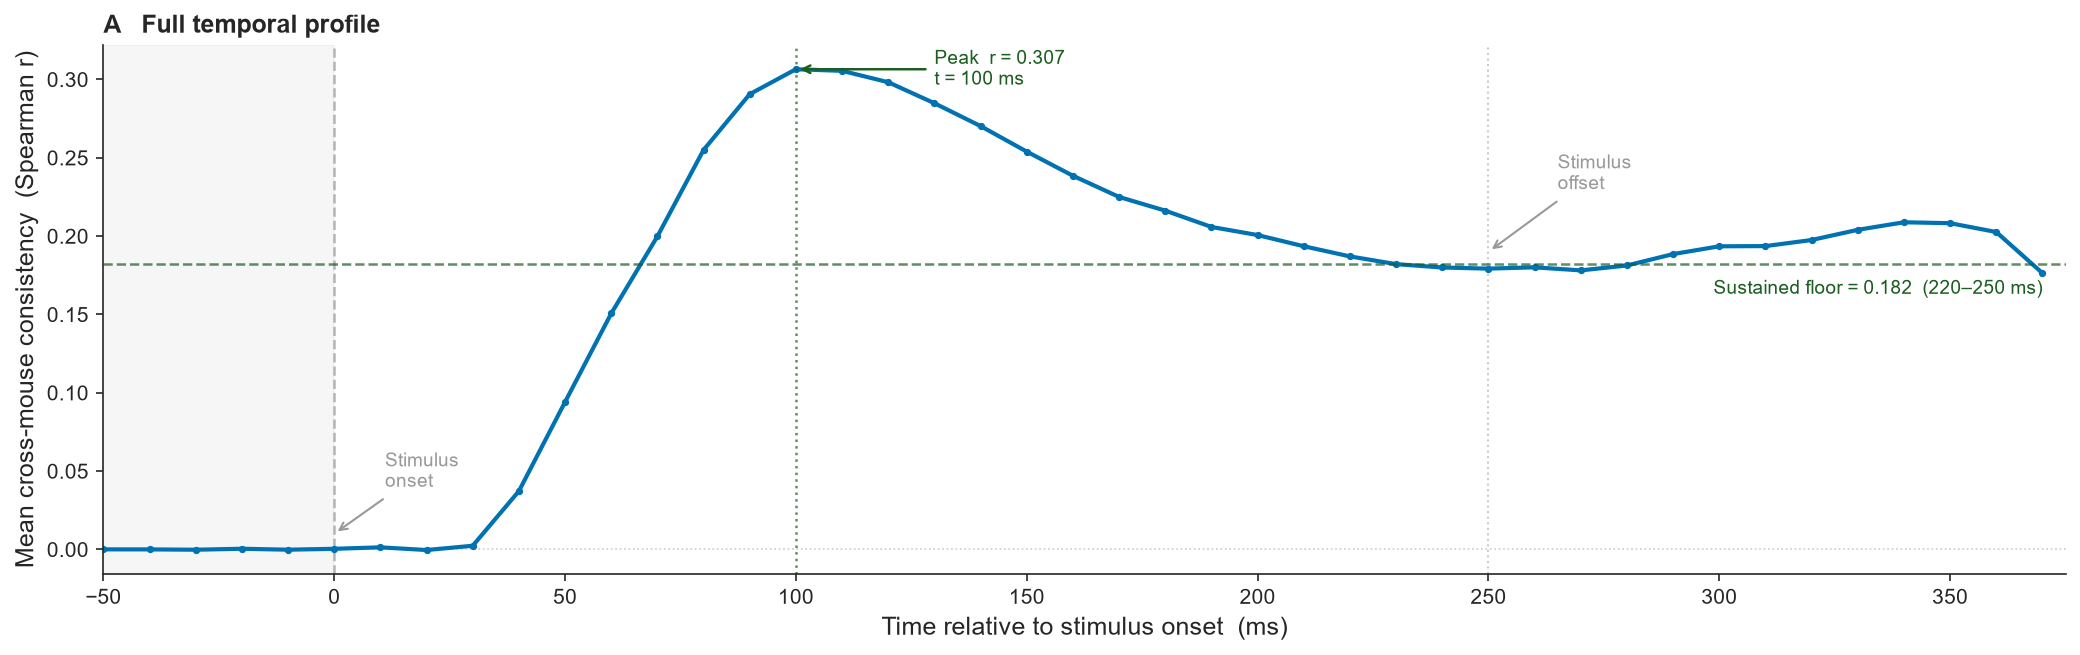
\includegraphics[width=\textwidth]{figures/fig3_temporal_profile.png}
  \caption{\textbf{Cross-mouse consistency follows a stereotyped
  two-component trajectory.}
  Mean cross-mouse consistency over time (25~ms windows, 10~ms steps,
  $n = 32$ mice; blue). Pre-stimulus baseline $\approx 4 \times 10^{-5}$.
  Onset: 50~ms; peak: $r = 0.307$ at 100~ms (green marker). Sustained
  floor: $r = 0.182$ (220--250~ms, shaded band and dashed horizontal
  line). Vertical dashed line: stimulus onset (0~ms); dotted line:
  stimulus offset (250~ms), beyond which back-to-back presentation
  creates contamination risk from the next image's V1 response
  ($\sim$290--300~ms onset).}
  \label{fig:temporal}
\end{figure}

\subsection{The transient peak coincides with a collapse of the shared
representation into a low-dimensional attractor}

To characterise the geometry of the shared representation at each time
point, we computed the participation ratio (PR) of the average cosine
similarity matrix across mice,
$\mathrm{PR} = (\sum_i \lambda_i)^2 / \sum_i \lambda_i^2$, where
$\lambda_i$ are the eigenvalues of that matrix, see Methods \ref{Methods:PR}; PR measures
effective dimensionality, from 1 (one dominant eigenvalue) to $n$
(uniform eigenvalues). Pre-stimulus PR was $\approx 108$, close to the
maximum of 118 possible, indicating an approximately uniform,
unstructured geometry at baseline. At the consistency peak (100~ms), PR
dropped to 31.5 --- the shared representation occupied only
$\approx$27\% of the available dimensions --- before partially
recovering to 61.2 by 250~ms (Fig.~\ref{fig:geometry}A). The same pattern
held when PR was computed within each mouse individually and only then
averaged, a measure that never involves cross-mouse averaging and is
therefore not confounded with consistency by construction (pre-stimulus
$\approx 35.6 \to$ peak 15.3 $\to$ 250~ms 24.4). Across the post-stimulus
epoch, PR and mean consistency were strongly anti-correlated for both the
averaged-matrix PR (Spearman $r = -0.853$, $p = 3.5 \times 10^{-6}$) and
the per-mouse PR ($r = -0.805$, $p = 3.2 \times 10^{-5}$): the moment of
maximal cross-mouse agreement is the moment of maximal representational
compression, even when compression is measured entirely within individual
mice.

Because the sliding windows overlap, the $n=19$ points entering this
correlation are not independent and the analytic $p$-values above
understate the true $p$-value. Recomputing on fully independent,
non-overlapping 30~ms-spaced windows (13 points, no shared spike-count
bins) confirmed the coupling under a conventional test requiring no
autocorrelation correction ($r = -0.929$, $p = 4.6 \times 10^{-6}$), see Methods \ref{Methods:PR}. A
circular-shift permutation test, and a control for a shared dependence on
the raw stimulus-evoked response envelope, gave consistent results and are
reported in the Supplementary Results
(\S\ref{supp:pr-envelope}); briefly, the PR--consistency coupling survived
partialling out the envelope essentially unchanged (partial
$r = -0.801$, avg-matrix), while the envelope's own link to consistency
did not survive the autocorrelation-robust test.

Eigendecomposition of the average similarity matrix at the 100~ms peak
showed a gradually decaying spectrum: the top 8 eigenvectors accounted for
35.2\% of variance (14.75\%, 4.60\%, 3.57\%, 3.21\%, 2.77\%, 2.12\%,
2.07\%, 2.07\% for dimensions 1--8; Fig.~\ref{fig:geometry}B). The two
dominant dimensions were interpretable in terms of low-level image
statistics --- Dim~1 as a signal-strength axis (correlated with response
magnitude, $r = +0.44$, and early CNN features) and Dim~2 as a
spatial-scale axis (correlated with sparsity, $r = -0.51$) --- while
overall cross-mouse consistency did not load strongly onto any single
eigenvector (maximum $|r| = 0.28$; Fig.~\ref{fig:geometry}C), consistent
with the shared structure being distributed across the compressed space
rather than concentrated along one axis. The full eigenvector-property
heatmap and an image gallery of the two dominant dimensions are in
Supplementary Fig.~\ref{fig:Seigen}--\ref{fig:Sattractor}.

\begin{figure}[htbp]
  \centering
  
\includegraphics[width=\textwidth]{figures/fig4_representational_geometry.png}
  \caption{\textbf{The consistency peak coincides with collapse into a
  low-dimensional attractor.}
  \textbf{(A)} Participation ratio (PR; right axis, light purple) and mean
  cross-mouse consistency (left axis, blue) co-plotted over time.
  Averaged-matrix PR: pre-stimulus $\approx 108$; peak-window PR $= 31.5$
  (27\% of available dimensions); 250~ms PR $= 61.2$. Per-mouse PR
  (shaded band, $\pm$ SEM): pre-stimulus $\approx 35.6$; peak-window
  PR $= 15.3$; 250~ms PR $= 24.4$. Post-stimulus Spearman
  $r(\text{PR, consistency})$ annotated for both the averaged-matrix PR
  ($-0.853$, $p = 3.5 \times 10^{-6}$) and the per-mouse PR ($-0.805$,
  $p = 3.2 \times 10^{-5}$).
  \textbf{(B)} Variance explained by the top 8 eigenvectors of the
  average cosine similarity matrix at 100~ms (bars, left axis;
  cumulative line, right axis; top 8 dims $= 35.2\%$ total).
  \textbf{(C)} Image layout in two-dimensional attractor space
  (Dim~1: signal-strength axis; Dim~2: sparsity axis), coloured by
  cross-mouse consistency.}
  \label{fig:geometry}
\end{figure}

\subsection{Fast-spiking units carry disproportionately more
cross-mouse-consistent signal than regular-spiking units}

To test whether distinct cell classes differentially produce the
transient and sustained components of consistency, we classified VISp
units by waveform trough-to-peak duration using a 2-component Gaussian
mixture model (GMM) fit in log-space to all 3,694 QC-passing units, see Methods
\ref{Methods:RSU_FSU}. Units were called fast-spiking (FSU) or regular-spiking (RSU)
only if their posterior class membership exceeded 0.9 \emph{and} they fell
within the central 90\% probability mass of that component, yielding
narrow/broad boundaries of 0.357~ms and 0.467~ms and classifying 634
units as FSU, 2,777 as RSU, and 283 (7.7\%) as ambiguous (excluded from
both classes).

We evaluated the FSU/RSU dissociation two ways: at the pooled-population
level, where response matrices combine many units per session, and at the
single-unit level, where each unit's own response is scored individually
against every other session's population, with no pooling or unit-count
confound at any step, see Methods \ref{Methods:RSU_FSU}. The single-unit approach is the more robust of the
two: pooled-population sessions must have $\geq$15 units of both classes,
restricting that analysis to 9/32 sessions and to comparisons sensitive to
between-class differences in unit count. After controlling for this by
subsampling each RSU session's units down to that session's own FSU count,
the pooled-population transient-to-sustained (T/S) ratio was
$2.02\times$ for matched RSU versus $2.12\times$ for FSU, in the same
direction as before matching (raw: $1.60\times$ vs.\ $2.12\times$); a
parallel session-level split on FSU fraction gave the same direction of
effect after an analogous unit-count control. Full pooled-population and
session-split results are in Supplementary Results
(\S\ref{supp:pooled-fsu}; Supp. Fig.~\ref{fig:Spoplevel}).

At the single-unit level, FSU units ($n = 368$) scored $\sim$1.9$\times$
higher than RSU units ($n = 1{,}499$) on cross-mouse consistency (FSU
median $= 0.087$, mean $= 0.095$; RSU median $= 0.046$, mean $= 0.052$;
Mann-Whitney $p = 1.4\times10^{-45}$; Fig.~\ref{fig:celltypes}B), with a
sharper transient shape (FSU T/S $= 3.62\times$; RSU T/S $= 2.65\times$;
Fig.~\ref{fig:celltypes}D). FSU units also had higher raw response
magnitude and lower lifetime sparseness than RSU units (both
$p < 10^{-300}$); the class-consistency relationship attenuated but
remained highly significant after partialling out both magnitude and
sparsity (raw Spearman $r = 0.328$, $p = 4.3\times10^{-48}$; partial
$r = 0.116$, $p = 5.4\times10^{-7}$), indicating the FSU advantage is not
simply a restatement of firing-rate differences.

To validate the waveform-based classification against ground truth, we
identified 18 optotagged VISp units across five Pvalb-IRES-Cre$\times$Ai32
sessions, see Methods \ref{Methods:Optotagging}. Sensitivity of the waveform classifier (PV$^+ \to$ GMM FSU) was
78\%, and precision (GMM FSU $\to$ PV$^+$) was 27\% --- typical of
duration-based interneuron classification generally
\citep[cf.][]{ye2025}. Scored individually, optotagged units fell at the
66th percentile of the waveform-inferred FSU distribution (median
$= 0.123$) with a T/S ratio of $3.18\times$, intermediate between the
waveform FSU and RSU single-unit curves (Fig.~\ref{fig:celltypes}B,D).

\begin{figure}[htbp]
  \centering
  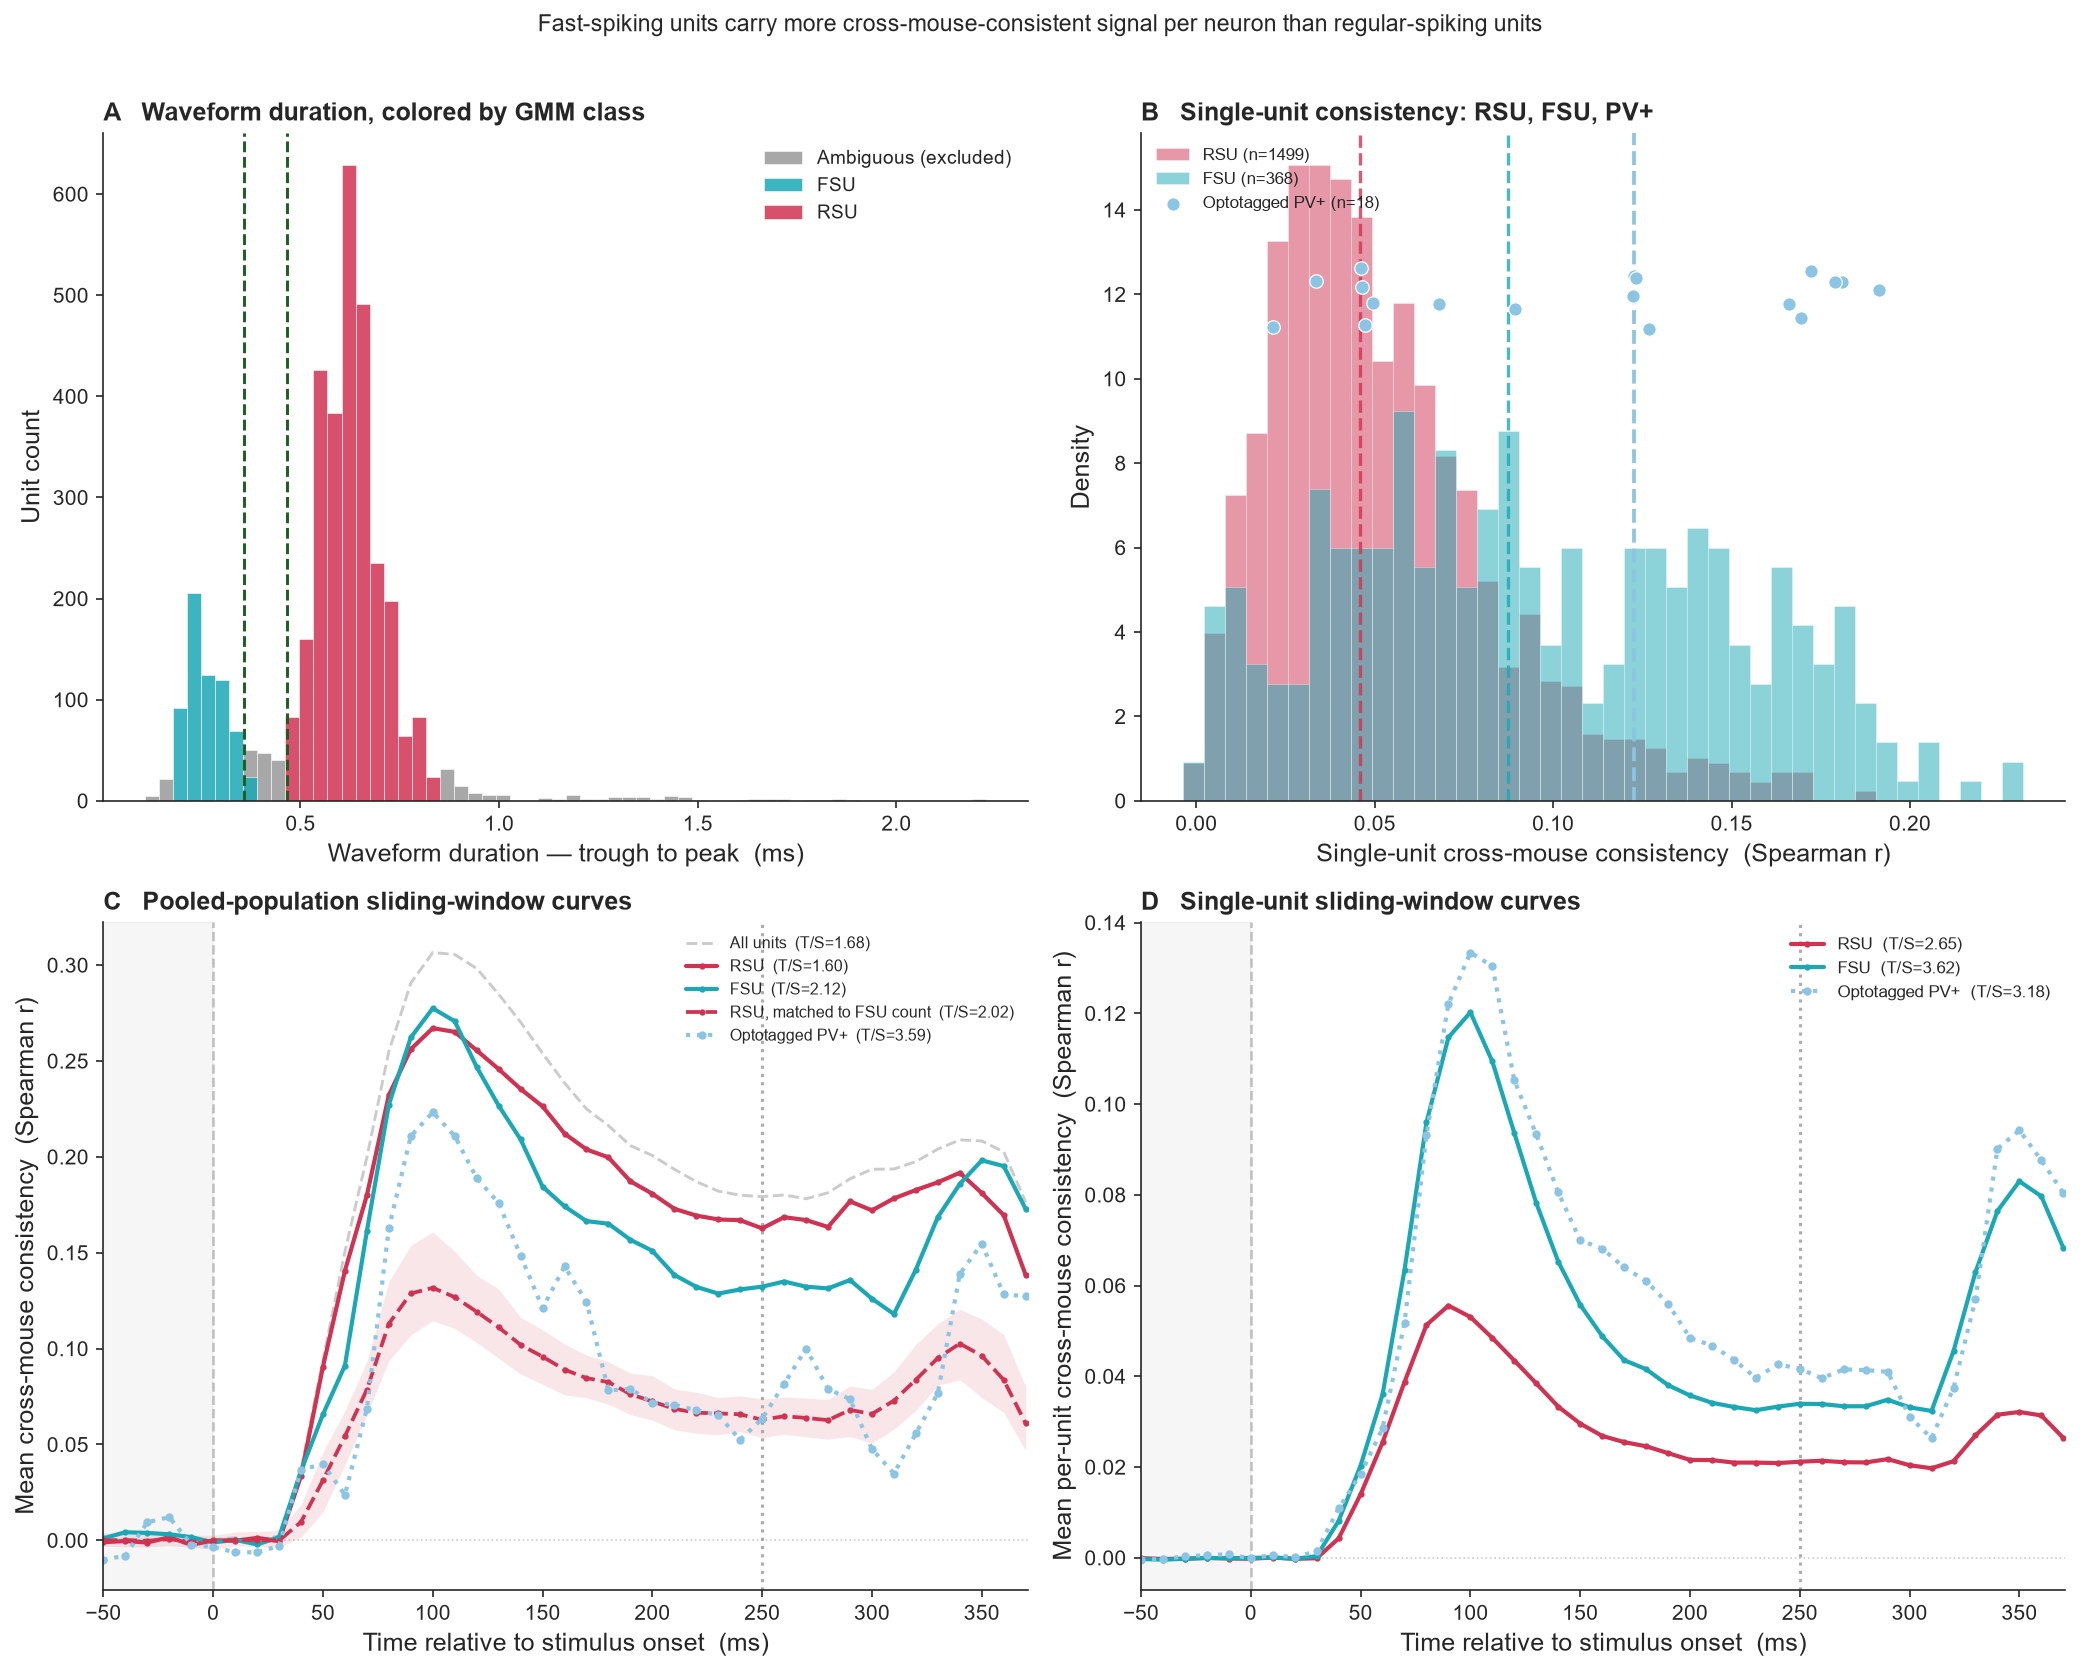
\includegraphics[width=\textwidth]{figures/fig5_cell_type_dissociation.png}
  \caption{\textbf{Fast-spiking units carry more cross-mouse-consistent
  signal per neuron than regular-spiking units, corroborated by
  genetically confirmed PV$^+$ interneurons.}
  \textbf{(A)} Waveform duration distribution across all 3,694
  QC-passing VISp units, colored by GMM classification: FSU (teal, $n =
  634$), RSU (pink, $n = 2{,}777$), and excluded ambiguous units (grey,
  $n = 283$). Dashed lines: narrow/broad classification boundaries
  (0.357~ms and 0.467~ms).
  \textbf{(B)} Single-unit cross-mouse consistency distributions for RSU
  ($n = 1{,}499$) and FSU ($n = 368$) units, with optotagged PV$^+$ units
  ($n = 18$, teal-blue circles) overlaid. Dashed vertical lines: class
  medians (RSU $= 0.046$; FSU $= 0.087$; PV$^+$ $= 0.123$).
  \textbf{(C)} Pooled-population sliding-window curves: all units (dashed
  grey), RSU (pink, T/S $= 1.60\times$), FSU (teal, T/S $= 2.12\times$),
  RSU subsampled to each session's own FSU count (pink dashed, T/S $=
  2.02\times$, shaded 95\% band), and optotagged PV$^+$ (teal-blue dotted,
  T/S $= 3.59\times$).
  \textbf{(D)} Single-unit sliding-window curves: RSU (pink, T/S $=
  2.65\times$), FSU (teal, T/S $= 3.62\times$), and optotagged PV$^+$
  (teal-blue dotted, T/S $= 3.18\times$).}
  \label{fig:celltypes}
\end{figure}

\subsection{FSU-gated shrinkage toward the population mean reproduces the
timing, but not the magnitude, of the dimensionality collapse}

The results above establish that the transient collapse in shared
dimensionality (\S2.3) and the disproportionate cross-mouse-consistent
signal carried by FSU units (\S2.4) co-occur, but do not test whether FSU
activity is mechanistically sufficient to produce the collapse itself. We
constructed a model in which each unit's response to each image is fixed at
its value in an early window (30--50~ms post-onset, before recurrent or
feedback contributions are thought to dominate; see Introduction) and is
then shrunk toward the per-image population mean by a time-varying factor
$\lambda(t)$:
\begin{equation}
  \lambda(t) = \lambda_\mathrm{max} \cdot \frac{g(t)}{\kappa + g(t)}, \qquad
  r_i(\mathrm{image}, t) = f_i(\mathrm{image}) - \lambda(t)\,
  \big[f_i(\mathrm{image}) - \bar{f}(\mathrm{image})\big],
\end{equation}
where $f_i(\mathrm{image})$ is unit $i$'s frozen early-window response,
$\bar{f}(\mathrm{image})$ is the per-image population mean across units in
that same window, and $g(t)$ is the measured FSU population cross-mouse
consistency curve (Fig.~\ref{fig:celltypes}C, teal curve), rescaled to
$[0,1]$. Neither $f_i$ nor $g(t)$ is fit; the only free parameters are
$\lambda_\mathrm{max}$ (the ceiling on shrinkage strength) and $\kappa$
(how quickly shrinkage approaches that ceiling as FSU activity rises).
Participation ratio was then computed from the resulting model responses
using the identical pipeline as the real data (\S2.3, Methods
\ref{Methods:PR}).

Because raw participation ratio computed from a small subset of sessions
reads systematically lower than the full-dataset value at every time point
(a known small-sample bias in this statistic, arising from noisier averaged
similarity matrices at low session counts), parameters were selected by
five-fold cross-validation across the 32 VISp sessions using a
shape-normalised $R^2$ (both model and held-out real curves min-max
normalised before comparison, restricted to the 0--250~ms window used
throughout this paper to avoid next-image contamination), rather than by
fitting the raw scale directly, see Methods \ref{Methods:Shrinkage}. This
selected $\lambda_\mathrm{max} = 0.9$ and $\kappa = 0.2$ in every fold (mean
held-out shape-$R^2 = 0.808 \pm 0.061$; Fig.~\ref{fig:shrinkage}D).

Applying these cross-validated parameters to the full dataset, the model
closely reproduces the \emph{timing} of the collapse and recovery
(shape-$R^2 = 0.995$; Fig.~\ref{fig:shrinkage}B) but substantially
underestimates its \emph{magnitude}: raw participation ratio drops to 31.4
in the data but only to 64.4 in the model (raw $R^2 = 0.204$;
Fig.~\ref{fig:shrinkage}A), despite both curves sharing a near-identical
pre-stimulus baseline ($\approx$108 vs.\ $\approx$101). FSU-gated shrinkage
toward the population mean therefore reproduces \emph{when} the population
code compresses, using only measured FSU activity and each unit's own
early, fixed tuning, but a single scalar shrinkage term is insufficient to
account for the full depth of compression observed.

\begin{figure}[htbp]
  \centering
  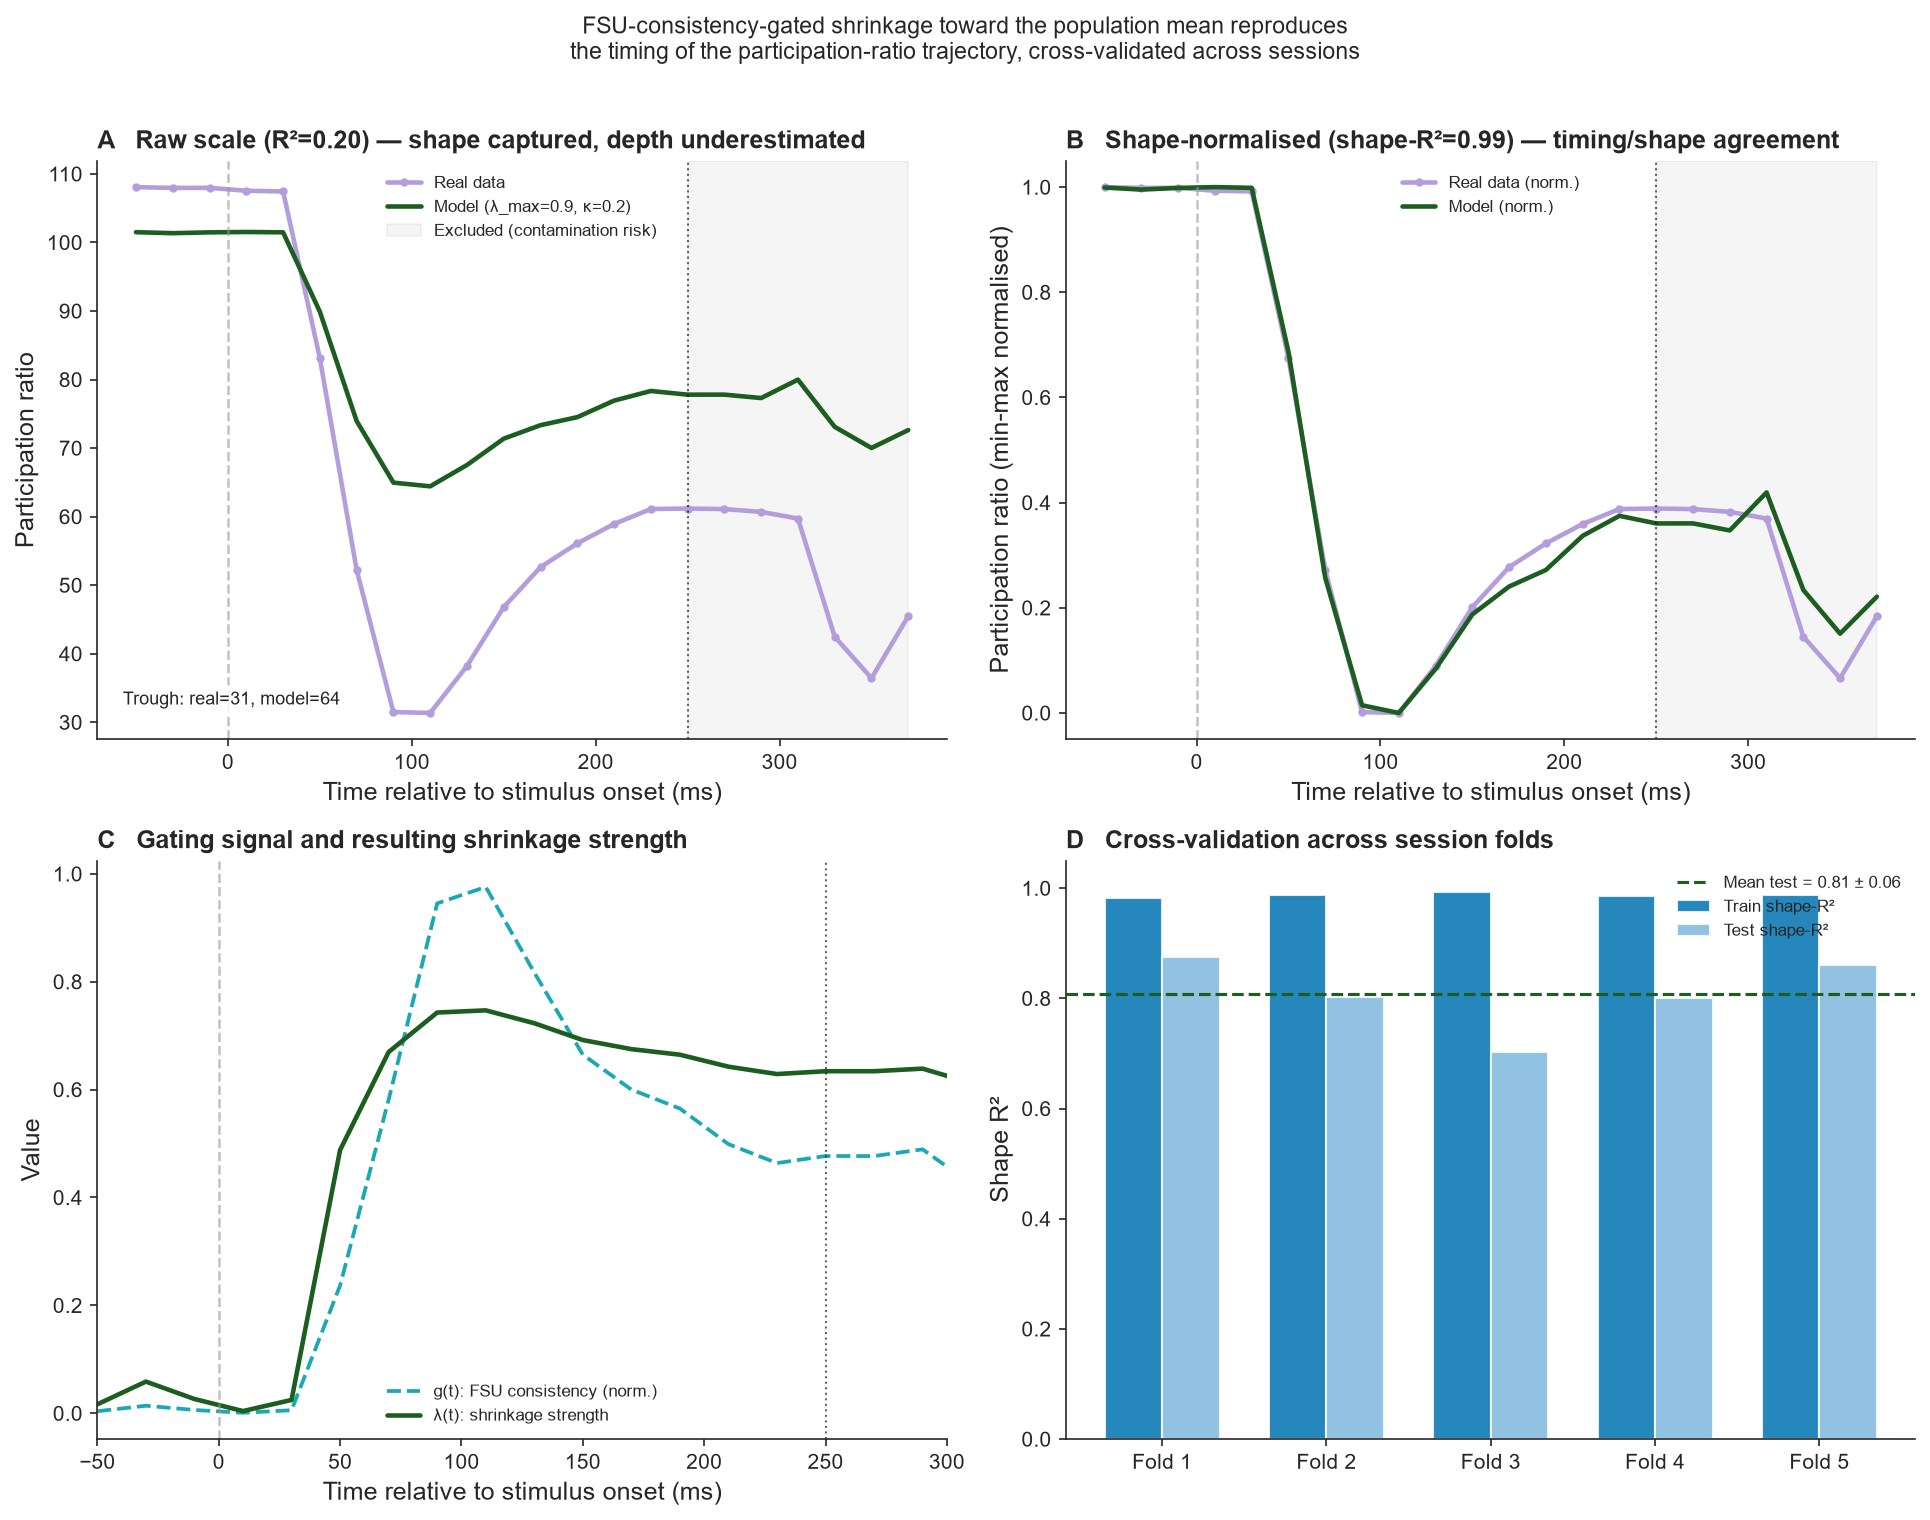
\includegraphics[width=\textwidth]{figures/fig6_pr_shrinkage_model.png}
  \caption{\textbf{FSU-consistency-gated shrinkage toward the population
  mean reproduces the timing, but not the magnitude, of the
  participation-ratio trajectory.}
  \textbf{(A)} Real (teal) and model (green) participation ratio on the raw
  scale. Both curves collapse and recover on a similar timescale; the model
  systematically underestimates collapse depth (real trough $=31.4$; model
  trough $=64.4$; raw $R^2 = 0.204$).
  \textbf{(B)} The same two curves after min-max normalisation within the
  0--250~ms window, isolating timing/shape agreement from absolute
  magnitude (shape-$R^2 = 0.995$).
  \textbf{(C)} The FSU gating signal $g(t)$ (dashed) and the resulting
  shrinkage strength $\lambda(t)$ (solid) under the cross-validated
  parameters ($\lambda_\mathrm{max}=0.9$, $\kappa=0.2$).
  \textbf{(D)} Five-fold cross-validation across VISp sessions: train
  (dark) and held-out test (light) shape-$R^2$ per fold, all folds
  selecting identical parameters; mean held-out shape-$R^2 = 0.808 \pm
  0.061$ (dashed line).}
  \label{fig:shrinkage}
\end{figure}

\subsection{Controls: adaptation and behavioural state do not explain the
results}

If mice habituated to images similarly over the session, or shared
transient arousal or locomotion states time-locked to particular images,
consistency could reflect shared history or state rather than shared
tuning. Splitting each session's trials chronologically, per-image
consistency was highly stable between early and late halves (Spearman
$r = 0.960$, $p = 6.1 \times 10^{-66}$; Fig.~\ref{fig:controls}A), with a
small mean difference in the direction opposite a shared-adaptation
confound ($+0.015$, $p = 1.1 \times 10^{-8}$), consistent instead with
modest non-selective fatigue. Neither the cross-mouse coefficient of
variation (CV) of pupil area ($r = +0.056$, $p = 0.55$, $n = 26$ sessions
with eye tracking) nor of running speed ($r = -0.033$, $p = 0.72$,
$n = 32$ sessions) predicted per-image consistency
(Fig.~\ref{fig:controls}B--C). Extended adaptation-control analyses,
including replication of the early/late split at the level of full
sorted curves, are in Supplementary Results
(\S\ref{supp:adaptation-extended}; Supp. Fig.~\ref{fig:Sadapt}).

\begin{figure}[htbp]
  \centering
  
\includegraphics[width=\textwidth]{figures/fig7_controls.png}
  \caption{\textbf{Cross-mouse consistency is not driven by shared
  adaptation, pupil-area fluctuations, or running-speed fluctuations.}
  \textbf{(A)} Per-image consistency in the chronologically early vs.\
  late trial half (scatter; dashed line: equal consistency). Spearman
  $r = 0.960$ ($p = 6.1 \times 10^{-66}$) across images.
  \textbf{(B)} Cross-mouse pupil-area CV vs.\ per-image consistency
  (Spearman $r = +0.056$, $p = 0.55$, $n = 26$ sessions with
  eye-tracking).
  \textbf{(C)} Cross-mouse running-speed CV vs.\ per-image consistency
  (Spearman $r = -0.033$, $p = 0.72$, $n = 32$ sessions).}
  \label{fig:controls}
\end{figure}

\subsection{The transient is specific to natural scenes}

Static gratings produced substantially higher absolute consistency than
natural scenes, see Methods \ref{Methods:Grating} (mean $r = 0.720$ vs.\ $r = 0.314$, fixed 0--250~ms
window; Fig.~\ref{fig:gratings}A), despite comparably high within-mouse
response reliability for both stimulus classes (gratings $0.992$, natural
scenes $0.978$), ruling out a reliability confound. The temporal
\emph{shape} nonetheless differed qualitatively: gratings rose by
$\sim$60~ms and then remained essentially flat (T/S $\approx 1.00\times$),
while natural scenes showed the characteristic transient-plus-sustained
structure (T/S $= 1.68\times$). Because gratings have only 30 conditions
against natural scenes' 118 images, and the Spearman consistency measure's
noise properties depend on this item count independently of any real
representational difference, we recomputed natural-scenes consistency
after subsampling to 30 images per draw to match the gratings item count
exactly (50 draws). This left both the magnitude ($r = 0.303$, 95\% range
$[0.258, 0.354]$, against $0.314$ unmatched) and the T/S ratio ($1.66\times$
vs.\ $1.68\times$ unmatched) essentially unchanged, confirming that
neither the higher absolute consistency nor the flatter temporal shape of
gratings is an artefact of their smaller stimulus set
(Fig.~\ref{fig:gratings}B--C).

\begin{figure}[htbp]
  \centering
  
\includegraphics[width=\textwidth]{figures/fig8_gratings_vs_natural_scenes.png}
  \caption{\textbf{Static gratings produce a weaker-transient but
  higher-magnitude cross-mouse consistency than natural scenes.}
  \textbf{(A)} Raw mean cross-mouse consistency over time for natural
  scenes (dark blue, peak $r = 0.307$ at 100~ms, T/S $= 1.68\times$) and
  static gratings (gold, rises by $\sim$60~ms then stays flat,
  T/S $\approx 1.00\times$). Light blue: natural-scenes consistency
  recomputed after subsampling to 30 images per draw (item-count-matched
  to gratings; peak $r = 0.291$, T/S $= 1.66\times$), closely tracking
  the full-118-image curve in shape.
  \textbf{(B)} Within-mouse response reliability distributions for
  natural scenes (mean $= 0.978$) and gratings (mean $= 0.992$): both
  near ceiling, so the consistency gap is not a reliability artefact.
  \textbf{(C)} Sorted per-item consistency in the fixed 0--250~ms window
  against rank fraction: natural scenes (full 118 images, mean
  $r = 0.314$), static gratings (30 conditions, mean $r = 0.720$), and
  natural scenes subsampled to 30 images per draw (mean of sorted curves
  $= 0.303$). Matching item count leaves the natural-scenes estimate
  essentially unchanged.}
  \label{fig:gratings}
\end{figure}

\subsection{Consistency is highest in V1, present but weaker in
thalamus, and absent outside the visual system}

Applying the same pipeline to five additional visual cortical areas
(VISl, VISal, VISpm, VISam, VISrl; 20--28 sessions each,
$\geq$10 QC-passing units per session) showed VISp had the highest peak
sliding-window consistency ($r = 0.307$) of the six cortical areas. The
five extrastriate areas were lower and broadly comparable to one another (VISl $r = 0.186$; VISal $r =
0.234$; VISpm $r = 0.210$; VISam $r = 0.238$; VISrl $r = 0.187$;
Fig.~\ref{fig:hierarchy}A), with transient-plus-sustained temporal
structure qualitatively present in all six areas. Reliability was high
and comparable across areas (0.964--0.978), so this ordering reflects
genuine differences in raw consistency rather than a reliability
confound.

Extending the pipeline to two thalamic structures --- lateral posterior
nucleus (LP) and dorsal lateral geniculate nucleus (LGd), the primary
feedforward relay to V1 --- showed that cross-mouse consistency is
already present at the thalamic stage but substantially lower than in
V1 (LP peak $r = 0.140$; LGd peak $r = 0.092$; Fig.~\ref{fig:hierarchy}B),
indicating that cortex adds representational structure beyond what is
inherited from thalamic input. Hippocampal area CA1, included as a
negative control, showed no stimulus-locked consistency at any time
point (peak $r = 0.002$), confirming the measure is specific to
visually-responsive structures rather than a generic property of neural
population recordings.

Because these nine areas differ systematically in per-session unit
count, which inflates raw consistency independently of any genuine
areal difference, we recomputed peak consistency after subsampling
every area's unit pool to a common count (39 units/session, the
smallest area's mean; 20 draws). The ordering among the six cortical
areas was materially unchanged; among the thalamic and hippocampal
areas, LGd's matched estimate closely tracked its raw value, while LP's
matched estimate should be interpreted cautiously given its smaller
session count (19) and correspondingly wider bootstrap interval (full
values in Methods \ref{Methods:QC}).

\begin{figure}[htbp]
  \centering
  
\includegraphics[width=\textwidth]{figures/fig9_cross_area_hierarchy.png}
  \caption{\textbf{Cross-mouse representational consistency is highest
  in V1, present but weaker in thalamus, and absent in a hippocampal
  control area.}
  \textbf{(A)} Temporal profiles of cross-mouse consistency for VISp
  and five extrastriate areas (VISl, VISal, VISpm, VISam, VISrl).
  Triangles: empirical peak per area; dashed lines: sustained floor
  (220--250~ms).
  \textbf{(B)} Temporal profiles for VISp alongside lateral posterior
  nucleus (LP) and dorsal lateral geniculate nucleus (LGd, the primary
  thalamic relay to V1) and hippocampal area CA1 (negative control).
  Consistency is present but substantially lower in both thalamic
  structures than in VISp, and indistinguishable from zero throughout
  the epoch in CA1. Legend values give raw peak and floor consistency
  per area; session counts vary by area (Methods \ref{Methods:QC}).}
  \label{fig:hierarchy}
\end{figure}

% ── Discussion ────────────────────────────────────────────────────────────────

\section{Discussion}

We have shown that mouse V1 does not represent natural images with a
constant degree of cross-individual agreement. Instead, it passes through
a transient, low-dimensional population state --- peaking at $\sim$100~ms
post-stimulus and visible directly in the participation ratio of the
shared representation --- and this transient state is precisely the
moment at which different animals' representations are most alike. This
is the strongest and most direct result in the paper, requiring no
cell-type classification, circuit model, or auxiliary assumptions: the
temporal profile is incompatible with either purely feedforward tuning (a
step function) or purely recurrent attractor dynamics (a sustained
plateau), and its peak coincides with a collapse of the shared geometry to
its minimum dimensionality. In the language of neural population geometry
\citep{chung2021}, stimulus onset transiently contracts the
representational space rather than adding a new, image-specific
direction to it. Such contraction is not specific to vision or to this
particular statistic: comparable stimulus-triggered reductions in
population dimensionality or trial-to-trial variability have been
reported across cortical areas, species, and recording modalities
\citep{churchland2010, mazzucato2016}. The coupling between dimensionality
and consistency is robust to three independent checks that rule out it
being merely definitional: it holds when PR is computed within each mouse
and only then averaged, it survives partialling out the shared
stimulus-evoked response envelope, and it holds on non-overlapping windows
that share no spike-count bins by construction.

The remaining results address why this compression occurs, and converge
on fast-spiking inhibition. Scored one neuron at a time, individual FSU
units carry roughly $1.9\times$ the cross-mouse-consistent signal of RSU
units, surviving controls for raw magnitude and sparsity and including a
sharper single-unit transient shape. Interneuron physiology offers
converging reasons to expect exactly this pattern: parvalbumin-expressing
interneurons pool broadly across the local excitatory population, tracking
the net tuning bias of their neighbours rather than a sharp, private
receptive field, so an averaged signal should by default vary less across
animals; they impose a largely divisive, gain-like transformation on
pyramidal output, consistent with the iceberg-style sharpening already
invoked to explain the transient's shape; and their recruitment, some
50--60~ms after the initial feedforward volley, is closer to the timescale
of feedback inhibition than to that earliest feedforward wave itself
\citep{kerlin2010, atallah2012, shapiro2022, troyer1998, lamme2000,
kirchberger2023, isaacson2011}. A recent preprint applying an analogous
consistency logic to the same 118-image stimulus set, recorded via
two-photon imaging across genetically-defined Cre lines, similarly finds
inhibitory (PV, SST, VIP) population geometry clustering by cell-type
identity almost independent of visual area, unlike excitatory geometry
\citep{toosi2025}. Within our own data this dissociation is corroborated by
pooled-population and optotagging analyses, the latter consistent with
the known, imperfect agreement between waveform-based and genetic
interneuron classification more generally \citep{ye2025}.

The FSU-gated shrinkage model provides a direct, cross-validated test of
whether FSU activity is mechanistically sufficient to produce the observed
dimensionality collapse, rather than merely correlated with it. Using only
each unit's fixed early tuning and the independently measured FSU
consistency curve, the model reproduces the collapse's timing with high
fidelity, generalising across held-out session folds. That it nonetheless
underestimates collapse magnitude by roughly half indicates FSU activity
gates a shrinkage process that contributes to, but does not by itself
generate, the full compression observed --- consistent with a role for
additional circuit contributions, such as recurrent excitatory dynamics
among RSU units, that are not represented in this minimal model. This
converging pattern, in which the timing but not the full magnitude of an
FSU-linked effect can be captured by the simplest sufficient mechanism, is
consistent with the broader iceberg-effect framing already invoked to
explain the transient's shape (\citep{shapiro2022, troyer1998}): inhibition
sculpts and times the compression, without being its sole source.

Our findings extend rather than contradict existing accounts of V1
population geometry. The high-dimensional spontaneous state we observe
matches the power-law eigenspectrum reported for V1 \citep{stringer2019},
and a bias-corrected re-analysis of that same dataset recovers a similarly
small number of dominant dimensions using an independent estimator
\citep{pospisil2025}. Decomposing a visual response by time, rather than
collapsing it into one window, reveals structure invisible to static
approaches --- a lesson also drawn from time-resolved RSA of human MEG,
which dissociates an early, transient representational component from a
later, more persistent one \citep{cichy2014}. Our RSA approach differs from
Procrustes alignment and hyperalignment \citep{williams2021, haxby2011} in
measuring agreement on representational \textit{structure} rather than the
orientation of neural axes; a within-mouse RDM-space reliability of
$r = 0.832$ against a mean cross-mouse consistency of $r = 0.314$ indicates
that a substantial share of the representational signal is nonetheless
shared across individuals. Finally, the feedforward/recurrent distinction
\citep{lamme2000} maps naturally onto our two-component profile: the
$\sim$100~ms transient falls within the early feedforward epoch, when
shared thalamic-driven tuning should be more stereotyped across
individuals than recurrent contributions shaped by individual experience.

The transient's absence for static gratings --- despite their higher
absolute consistency but near-immediate plateau rather than a
transient-plus-sustained profile --- fits a broader literature in which
sparsification and decorrelation in V1 are engaged by natural-scene
statistics specifically, demonstrated via nonclassical receptive-field
manipulations in macaque V1, movie-versus-control comparisons in mouse V1,
and parametric removal of natural-scene spatial correlations in mouse V1
\citep{vinje2000, froudarakis2014, rikhye2015}. It is the specific
statistical structure of natural images, not stimulus complexity in some
more general sense, that appears to recruit the compression we observe;
gratings, though densely and reliably encoded, may simply not engage the
mechanism.

Taken together, these findings establish the transient compression of the
V1 population code as a measurable, reproducible, and --- in our data ---
mechanistically interpretable property of the visual response, with a
circuit mechanism that the cross-validated E/I model suggests is a stable
property of the mouse V1 architecture rather than an idiosyncrasy of the
32 mice sampled. If the shared geometry of V1 is transiently imposed by
inhibitory interneurons during a 50--150~ms window after stimulus onset,
downstream areas reading out V1 during this window receive a cleaner, more
stereotyped signal than at other times; such temporal gating of canonical
representational structure may be a general principle of cortical
computation, specifically engaged by complex, naturalistic stimuli rather
than by visual stimulation as such. A recent review of response
sub-additivity and variability quenching in visual cortex closes by
proposing population-level geometry as the natural next extension of
exactly this literature \citep{goris2024}; the present results, linking a
moment of dimensionality collapse to a moment of maximal cross-individual
agreement, are one instance of what that extension can look like.

% ── Methods ───────────────────────────────────────────────────────────────────
\section{Methods}

\subsection{Dataset}
\label{Methods:Dataset}

All data were obtained from the Allen Brain Observatory Visual Coding
Neuropixels dataset \citep{siegle2021}, accessed via the AllenSDK
(version~2.x). We used all 32 sessions of type
\textit{brain\_observatory\_1.1}, in which head-fixed mice passively
viewed a standardised battery of natural and artificial stimuli while six
Neuropixels probes recorded simultaneously from multiple visual areas.
The natural scenes stimulus (118 greyscale images, 250~ms per image, 50
repetitions per image, back-to-back with no inter-stimulus interval) and
the static gratings stimulus (orientation $\times$ spatial-frequency
conditions, 250~ms per presentation) were used. All analyses used the
VISp area designation from the Allen Common Coordinate Framework~v3 for
the main analysis; the cross-area analysis additionally included five
extrastriate cortical areas (VISl, VISal, VISpm, VISam, VISrl), two
thalamic structures (LP, LGd), and hippocampal area CA1 as a negative
control. There is one session per mouse in this dataset,
so ``32 mice'' and ``32 sessions'' are used interchangeably, and sessions
are the resampling/held-out unit in the cluster bootstrap and
cross-validation procedures below.

\subsection{Unit quality control}
\label{Methods:QC}

Units were retained if amplitude cutoff $< 0.1$, presence ratio $> 0.9$,
and ISI violation rate $< 0.5$. Sessions were included in the analysis of
a given area only if they contributed $\geq$10 QC-passing units in that
area. All 32 sessions met this threshold for VISp (range: 14--110 units).
Session counts for other areas were: VISl 24, VISal 23, VISpm 20,
VISam 26, VISrl 28, LP 19, LGd 16, CA1 25; mean units/session: VISp
63.0, VISl 38.9, VISal 67.1, VISpm 44.0, VISam 57.9, VISrl 50.5, LP
75.6, LGd 55.0, CA1 97.4. To control for the resulting SNR confound in
cross-area comparisons, each area's unit pool was randomly subsampled
to 39 units/session (VISl's mean, the smallest of the nine) over 20
draws, and the sliding consistency curve was recomputed on each matched
draw (raw $\to$ matched peak: VISp $0.307 \to 0.273$; VISl $0.186 \to
0.195$; VISal $0.234 \to 0.205$; VISpm $0.210 \to 0.240$; VISam $0.238
\to 0.195$; VISrl $0.187 \to 0.176$; LP $0.140 \to 0.112$; LGd $0.092
\to 0.087$; CA1 $0.002 \to 0.001$).

\subsection{Preprocessing and response matrix construction}
\label{Methods:Preprocessing}

Spike times were binned into 1~ms bins spanning $-75$ to $+404$~ms
relative to stimulus onset and stored as a tensor of shape (images
$\times$ units $\times$ bins) per session. Any response window
$[t_\mathrm{lo}, t_\mathrm{hi})$~ms was reconstructed by summing the
relevant bin columns, then z-scoring per unit across images.

\subsection{Within-mouse reliability}
\label{Methods:Within-mouse reliability}

Within-mouse split-half reliability was estimated by randomly
partitioning each image's 50 trials into two halves, computing the mean
population response vector for each half, and measuring their Spearman
rank correlation, repeated over 20 splits and Spearman-Brown corrected
\citep{spearman1910,brown1910}. This response-vector reliability is a QC
diagnostic computed in a different space than consistency (raw per-unit
response vectors vs.\ image-by-image similarity structure) and is not
used to normalise it. A directly comparable RDM-space reliability was additionally computed by splitting each mouse's
trials in half, converting each half to a similarity matrix, and
Spearman-correlating the two per-mouse matrices exactly as consistency
correlates two different mice's matrices, then Spearman-Brown correcting
and averaging over 20 splits and mice.

\subsection{Representational similarity analysis and cross-mouse
consistency}
\label{Methods:RSA}

For each session, the inter-image cosine similarity matrix was computed
from the z-scored response matrix:
$S_{ij} = \mathbf{x}_i \cdot \mathbf{x}_j /
(\|\mathbf{x}_i\| \|\mathbf{x}_j\| + \epsilon)$, $\epsilon = 10^{-8}$.
Per-image cross-mouse consistency was the mean Spearman rank correlation,
across all mouse pairs $(a,b)$, between their row-wise similarity profiles
for each image \citep{kriegeskorte2008}. Cluster bootstrap confidence
intervals resampled whole mice (not pairs) with replacement for 1000
iterations; pairs consisting of two copies of the same resampled mouse
were excluded to prevent spurious self-correlation.

\subsection{Sliding-window temporal analysis}
\label{Methods:Sliding window}

The RSA pipeline was repeated in 25~ms windows stepped at 10~ms
increments from $-50$ to $+370$~ms. Response matrices were z-scored
independently within each window. The sustained floor was estimated from
the 220--250~ms window only, to avoid contamination from the subsequent
image's response (back-to-back presentation places the next image's onset
response at $\sim$290--300~ms). Onset was defined as the first
post-stimulus window where mean consistency exceeded
$\max(2 \times \text{baseline},\, 0.05)$.

\subsection{Participation ratio and its controls}
\label{Methods:PR}

The PR of a positive semi-definite matrix with eigenvalues
$\lambda_i \geq 0$ is $\mathrm{PR} = (\sum_i \lambda_i)^2 /
\sum_i \lambda_i^2$ \citep{gao2017}, computed both on the cross-mouse
averaged similarity matrix and, separately, as the mean of each session's
own PR (20~ms grid). Because overlapping sliding windows are not
statistically independent, PR--consistency and PR--envelope correlations
were additionally assessed with a circular-shift permutation test (shifting
one series relative to the other at every non-trivial lag, which preserves
each series' own autocorrelation while destroying only their mutual
alignment) and with a fully independent, non-overlapping-window control
(30~ms spacing, no shared spike-count bins). A response-envelope proxy
(mean raw, pre-z-score population response per window) was used to test
whether the PR--consistency coupling reflected a shared dependence on
overall response magnitude, via the Spearman partial correlation
$r_{xy \cdot z} = (r_{xy} - r_{xz} r_{yz}) /
\sqrt{(1 - r_{xz}^2)(1 - r_{yz}^2)}$, with significance assessed both
analytically and via the circular-shift procedure above.

\subsection{Waveform-based cell class classification and single-unit
consistency}
\label{Methods:RSU_FSU}

Units were classified as FSU or RSU using trough-to-peak waveform
duration \citep{bartho2004,mccormick1985}, via a 2-component Gaussian
mixture model \citep{trainito2019} fit in log-space to all 3,694
QC-passing VISp units. A unit was assigned to a class only if its
posterior membership probability exceeded 0.9 \emph{and} it fell within
the central 90\% probability mass of that component (1.645 SD in
log-space); units failing either criterion were labelled ambiguous and
excluded. For pooled-population analyses, sessions with $<$15 QC-passing
units of both classes were excluded (9/32 sessions retained), and each
RSU session's pool was additionally subsampled to that session's own FSU
count over 50 draws to control for the within-session unit-count
difference. For single-unit consistency, each QC-passing unit's response
was treated as an $n=1$ population, rank-transformed and compared against
every \emph{other} session's full population profile, with no pooling or
unit-count confound at any step; magnitude and lifetime sparseness
(Rolls--Tovee measure) were computed from the same unit's raw spike counts
for the confound-control analysis.

\subsection{Optotagging}
\label{Methods:Optotagging}

Genetically confirmed PV$^+$ units were identified from the five
Pvalb-IRES-Cre/wt$\times$Ai32(RCL-ChR2(H134R)\_EYFP)/wt \citep{madisen2012}
sessions using single-pulse optotagging \citep{lima2009,cardin2010}. QC-passing
VISp units were classified as optotagged PV$^+$ if mean spike count in the
0--5~ms post-pulse window exceeded 0.05 spikes/pulse and the
light-to-baseline ratio exceeded 2.0 (baseline: 5~ms pre-pulse window);
the 5~ms window excludes polysynaptic responses. Sessions with $<$3
optotagged VISp units were excluded from pooled-population optotagged
curves.

\subsection{FSU-gated population-mean shrinkage model}
\label{Methods:Shrinkage}

For each session, each unit's raw (summed, non-z-scored) spike count per
image was computed in a fixed 30--50~ms window post-stimulus-onset
($f_i(\mathrm{image})$), and the per-image mean across units in that same
window was computed as the shrinkage target
($\bar{f}(\mathrm{image})$). At each subsequent time window $t$, a model
response matrix was constructed as $f_i(\mathrm{image}) -
\lambda(t)[f_i(\mathrm{image}) - \bar{f}(\mathrm{image})]$, where
$\lambda(t) = \lambda_\mathrm{max} \cdot g(t) / (\kappa + g(t))$ and $g(t)$
is the pooled-population FSU cross-mouse consistency curve (\S2.4,
Methods \ref{Methods:RSU_FSU}), min-max normalised to $[0,1]$ across the
full sliding-window epoch. Model response matrices were z-scored per unit
across images, identically to real response matrices (Methods
\ref{Methods:Preprocessing}), and participation ratio was computed from the
resulting cross-session-averaged cosine similarity matrix using the
identical procedure as the real data (Methods \ref{Methods:PR}).

Parameters $\lambda_\mathrm{max} \in \{0.90, 0.95, 0.97, 0.99, 0.995,
0.999\}$ and $\kappa \in \{0.05, 0.08, 0.1, 0.12, 0.15, 0.2\}$ were
selected by five-fold cross-validation (\texttt{scikit-learn}
\texttt{KFold}, shuffled, seed 42) over the 32 VISp sessions. Within each
fold, the parameter pair maximising shape-$R^2$ (Pearson-based $R^2$
computed after independently min-max normalising both the model and the
real participation-ratio curves within the 0--250~ms window) on the
training sessions was selected and evaluated on the held-out test
sessions using the same metric. Shape-normalisation was used rather than
raw-scale $R^2$ because participation ratio computed from a reduced number
of sessions is systematically biased downward relative to the full-dataset
value at every time point, independent of model correctness; shape-$R^2$
isolates timing/shape agreement from this scale bias. The parameter pair
selected in a majority of folds was applied to the full 32-session dataset
to obtain the reported fit.

\subsection{Grating response matrices}
\label{Methods:Grating}

Grating conditions were defined as unique (orientation, spatial
frequency) pairs present in all 32 sessions (30 conditions). The same QC
thresholds, z-scoring, and RSA pipeline were applied as for natural
scenes. For the item-count control, natural-scenes consistency was
recomputed after subsampling to 30 images per draw (50 draws), matching
the gratings condition count, for both the fixed 0--250~ms window and the
full sliding-window profile.

\subsection{Statistical tests}

Spearman rank correlation was used throughout for robustness to outliers
and bounded values. Wilcoxon signed-rank tests were used for paired
comparisons. No multiple-comparisons correction was applied to the two
pre-specified behavioural-state tests (pupil and running CV), which are
independent by construction. All bootstrap confidence intervals used 1000
iterations. The global random seed was 42, passed explicitly to all
stochastic operations.

\subsection{Data and code availability}

All neural data are publicly available through the Allen Brain Observatory
(\url{https://portal.brain-map.org}) and accessed using the AllenSDK
Python package. Analysis code is available at
\url{https://github.com/Jana-HQ/cross-mouse-v1-rsa}.

\subsection{AI use disclosure}

Claude Sonnet 5 (Anthropic) was used at several stages of this project.
In code development, it assisted with drafting and debugging analysis
scripts; all code was reviewed, tested, and validated by the author
against the underlying data and statistical methods described above, and
the author takes full responsibility for its correctness. In literature
search, it assisted in identifying and locating relevant prior work,
which the author then independently retrieved, read, and verified before
citation. In manuscript preparation, it assisted with drafting,
structuring, and editing text; all scientific content, interpretations,
claims, and conclusions are the author's own, and the author reviewed and
takes full responsibility for the accuracy and integrity of the final
manuscript. AI was not used to generate, analyze, or interpret primary
research data.

% ── Acknowledgements ──────────────────────────────────────────────────────────
\section*{Acknowledgements}

I thank the Allen Institute for Brain Science for making the Visual Coding
Neuropixels dataset publicly available, and Drs. Carsen Stringer and
Tahereh Toosi for helpful inputs. This research did not receive any specific
grant from funding agencies in the public, commercial, or not-for-profit
sectors.

% ── Competing interests ───────────────────────────────────────────────────────
\section*{Competing interests}

The author declares no competing interests.

% ══════════════════════════════════════════════════════════════════════════════
% ── Supplementary Information ────────────────────────────────────────────────
% ══════════════════════════════════════════════════════════════════════════════
\clearpage
\section*{Supplementary Information}

The sections below report analyses that support, replicate, or stress-test
claims made in the main text, but whose omission does not change the
paper's conclusions. Cross-references from the main text point here for
full statistical detail.

\subsection*{Image-level predictors of consistency}
\label{supp:predictors}

Response sparsity (fraction of units responding below the per-mouse
median $|z|$) was the strongest image-level predictor of cross-mouse
consistency (Spearman $r = -0.470$, $p = 7.8 \times 10^{-8}$), with
response magnitude a weaker positive predictor ($r = +0.276$,
$p = 2.5 \times 10^{-3}$; Supp. Fig.~\ref{fig:Spredictors}A--B). A
ResNet50 CNN feature embedding \citep{he2016}, pretrained on ImageNet
\citep{deng2009}, also predicted consistency in leave-one-out ridge
regression \citep{hoerl1970}; layer~2 (512-dimensional) gave the best
accuracy (LOO Pearson $r = -0.496$, $p = 1.1 \times 10^{-8}$) and was
selected as the primary CNN predictor, with the final layer
(1000-dimensional) performing comparably ($r = -0.486$,
$p = 2.5 \times 10^{-8}$; Supp. Fig.~\ref{fig:Spredictors}C).

The primary test of whether this CNN-based signal is subsumed by sparsity
was a nested $R^2$ model comparison rather than a partial correlation,
since it does not require residualising a fitted, cross-validated
prediction against the variable it was fit to predict. Adding the CNN
prediction to a sparsity-only model ($R^2 = 0.269$) raised $R^2$ to 0.453
for layer~2 ($\Delta R^2 = +0.184$) and to 0.374 for the final layer
($\Delta R^2 = +0.105$; Supp. Fig.~\ref{fig:Spredictors}D). As a secondary
check, added-variable (OLS) partial correlation, controlling for
sparsity, gave $r_\mathrm{partial} = -0.501$ (layer~2) and $-0.378$
(final layer). A second, non-parametric partialling method
(rank-residualised Spearman correlation) gave a substantially
larger-magnitude partial correlation for both layers
($r_\mathrm{partial} = -0.828$, $p = 5.5\times10^{-31}$ for layer~2;
$-0.887$, $p = 9.9\times10^{-41}$ for the final layer;
Supp. Fig.~\ref{fig:Scnn}C). This magnitude jump across partialling
methods is a signature of sparsity acting as a partial suppressor --- it
shares variance with both consistency and the CNN prediction, so removing
it from both can inflate residual alignment 
(Supp. Fig.~\ref{fig:Scnn}D). Galleries of the most and least
consistently represented images (Supp. Fig.~\ref{fig:Sgallery}) confirm
the sparsity relationship qualitatively: high-consistency images tend to
be dense, textured, and spatially distributed, while low-consistency
images tend to be dominated by a single salient, spatially compact
feature.

\subsection*{Robustness of the temporal profile: early/late windows,
rank stability, and second-order RSA}
\label{supp:temporal-robustness}

A coarser, non-overlapping two-window split (early: 0--75~ms; late:
75--250~ms) corroborates the sliding-window transient independently of
its 10~ms-step, overlapping-window construction: mean consistency was
substantially higher late than early (0.320 vs.\ 0.084, Wilcoxon
$p = 4.2 \times 10^{-21}$), with image rankings partially preserved
across the split (Spearman $r = 0.365$; Supp. Fig.~\ref{fig:Searlylate}).

Image-ranking stability was assessed by Spearman-correlating per-image
consistency across six representative epochs ($-25$, 25, 50, 100, 175,
250~ms). Rankings were near-zero before 50~ms and between the pre-stimulus
baseline and any post-stimulus epoch, but became substantially correlated
from 50~ms onward and highly correlated between the peak and sustained
epochs (100 vs.\ 250~ms: $r = 0.652$), indicating the transient and
sustained components are built substantially from the same set of
strongly-represented images rather than different image content at
different times (Supp. Fig.~\ref{fig:Srank}).

Second-order RSA scores cross-mouse agreement not on a single window's
similarity structure but on each image's full representational-dynamics
profile --- its similarity to all other images across five time windows.
This recovered a mean second-order $r = 0.187$ across images and a
temporal peak at exactly 100~ms, matching the first-order peak. Because
second-order $r$ correlates with first-order consistency at $r = 0.950$
across images ($p = 2.4\times10^{-60}$), it is best read as a related
re-parameterisation of the same underlying signal (Supp. Fig.~\ref{fig:Ssecondorder}).

\subsection*{PR--envelope control}
\label{supp:pr-envelope}

Because both PR and consistency are computed from the same per-window
response matrices, and both are weak pre-stimulus and late but strong near
the transient peak, we tested whether their coupling reflects a shared
dependence on the stimulus-evoked response envelope rather than a specific
dimensionality--agreement link. The envelope (mean raw, pre-z-score
population response per window) itself correlated with both consistency
($r = 0.525$, analytic $p = 0.021$) and PR (avg-matrix: $r = -0.711$,
$p = 6.5\times10^{-4}$; per-mouse: $r = -0.653$, $p = 2.5\times10^{-3}$).
Under the autocorrelation-robust circular-shift test, the
envelope--consistency correlation is no longer distinguishable from
chance ($p = 0.211$), while the PR--envelope correlations remain at the
floor $p$-value achievable given $n = 19$ independent windows
($p = 0.053$). The PR--consistency
coupling itself survived partialling out the envelope essentially
unchanged (avg-matrix: partial $r = -0.801$, analytic $p = 6.5\times10^{-5}$,
circular-shift $p = 0.053$; per-mouse: partial $r = -0.718$, analytic
$p = 8.0\times10^{-4}$, circular-shift $p = 0.053$; vs.\ raw
$r = -0.805$), indicating PR tracks consistency well beyond what the
response envelope predicts on its own.

\subsection*{Pooled-population and session-level FSU/RSU analyses}
\label{supp:pooled-fsu}

At the pooled-population level (sessions with $\geq$15 units of both
classes, 9/32 sessions), raw T/S was $1.60\times$ for RSU (peak $=
0.267$, sustained $= 0.167$) and $2.12\times$ for FSU (peak $= 0.277$,
sustained $= 0.131$). Because RSU sessions have far more units than FSU
sessions, which inflates similarity-matrix SNR independently of any
genuine cell-type effect, each RSU session's pool was subsampled to that
session's own FSU count (50 draws): the matched RSU T/S ratio narrowed to
$2.02\times$ (draw mean $2.05\times$, 95\% range $1.72$--$2.44\times$)
without eliminating the gap to FSU's $2.12\times$, though with only 9
sessions this comparison alone is not conclusive
(Supp. Fig.~\ref{fig:Spoplevel}, panel 1).

A parallel session-level analysis split sessions at the median FSU
fraction into high ($n = 16$, mean fraction 0.273, T/S $= 1.82\times$)
and low ($n = 16$, mean fraction 0.157, T/S $= 1.58\times$) groups,
showing the same direction of effect, which persisted after subsampling
the low-FSU group to the high-FSU group's mean unit count (T/S $=
1.69\times$; Supp. Fig.~\ref{fig:Spoplevel}, panel 1).

At the pooled-population level, the three-session optotagged PV$^+$ group
(sessions with $\geq$3 optotagged units) showed a sharper transient (T/S
$= 3.59\times$; peak $= 0.223$, sustained $= 0.062$) than waveform-inferred
FSU (T/S $= 2.12\times$), consistent with residual RSU/ambiguous
contamination in the waveform classification (3 of 18 optotagged units
fall in the confidently-RSU range) deflating the waveform-based pooled
estimate relative to the genetically confirmed one
(Supp. Fig.~\ref{fig:Spoplevel}, panels 2--3). Panel 4 shows single-unit
consistency vs.\ raw response magnitude by cell class, the scatter
underlying the magnitude/sparsity confound-control analysis in the main
text.

\subsection*{Adaptation control, extended}
\label{supp:adaptation-extended}

The distribution of per-image (early $-$ late) consistency differences
was centred slightly positive (mean $= +0.015$, one-sample $t$-test
$p = 1.1 \times 10^{-8}$), and both the early-half and late-half
per-image consistency curves closely tracked full-session consistency
($r = 0.985$ and $r = 0.984$ respectively), confirming that image rankings
are stable across trial halves and that the small absolute attenuation
late in the session is consistent with non-selective neural fatigue
rather than any consistency-relevant adaptation
(Supp. Fig.~\ref{fig:Sadapt}).

% ── Supplementary Figures ──────────────────────────────────────────────────────
\clearpage
\section*{Supplementary Figures}
\setcounter{figure}{0}
\renewcommand{\thefigure}{S\arabic{figure}}

\begin{figure}[htbp]
  \centering
  
\includegraphics[width=\textwidth]{figures/fig2_image_predictors.png}
  \caption{\textbf{Response sparsity and CNN-layer features each explain
  distinct variance in cross-mouse consistency.}
  \textbf{(A)} Consistency vs.\ response sparsity (fraction of units
  below per-mouse median $|z|$; Spearman $r = -0.470$,
  $p = 7.8 \times 10^{-8}$). Line: linear reference fit.
  \textbf{(B)} Consistency vs.\ mean $|$z-scored response$|$
  (Spearman $r = +0.276$, $p = 2.5 \times 10^{-3}$).
  \textbf{(C)} LOO Pearson $r$ per ResNet50 layer (purple: layer~2,
  the primary CNN predictor; teal: the final layer, the secondary
  predictor; grey: other layers).
  \textbf{(D)} Nested $R^2$: a sparsity-only model ($R^2 = 0.269$)
  compared against sparsity~$+$~layer~2 ($R^2 = 0.453$,
  $\Delta R^2 = +0.184$) and sparsity~$+$~final layer ($R^2 = 0.374$,
  $\Delta R^2 = +0.105$). This model-comparison statistic, rather than
  the partial-correlation coefficient, is the primary evidence that CNN
  features add explanatory power beyond sparsity; partial-correlation
  estimates, which vary substantially with partialling method, are
  reported as a robustness check in Supp. Fig.~\ref{fig:Scnn}.}
  \label{fig:Spredictors}
\end{figure}

\begin{figure}[htbp]
  \centering
  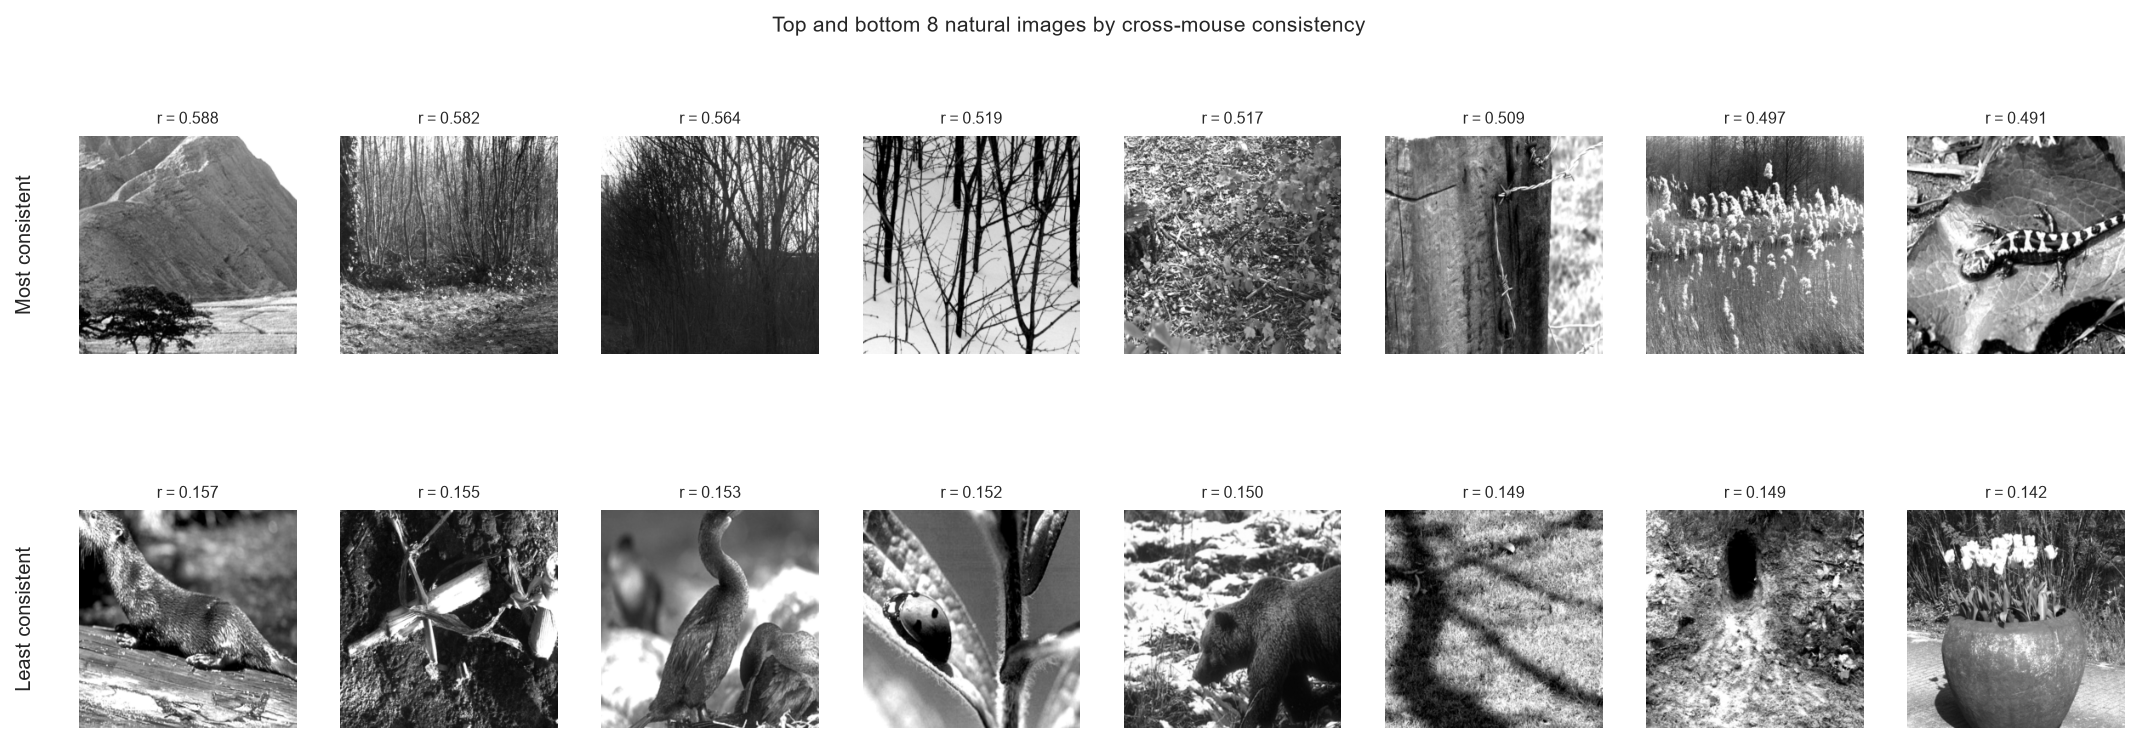
\includegraphics[width=\textwidth]{figures/figS1_image_gallery.png}
  \caption{\textbf{Gallery of high- and low-consistency natural images.}
  Top and bottom 8 images ranked by cross-mouse consistency. Consistency
  values shown in subtitles. High-consistency images tend to be dense
  and spatially distributed; low-consistency images tend to contain a
  single dominant feature against a background. This is a qualitative
  illustration; no statistical test is performed on image content.}
  \label{fig:Sgallery}
\end{figure}

\begin{figure}[htbp]
  \centering
  
\includegraphics[width=\textwidth]{figures/figS2_cnn_detail.png}
  \caption{\textbf{Partial-correlation robustness checks for the
  CNN--sparsity relationship, layer~2 and the final ResNet50 layer ---
  see Supp. Fig.~\ref{fig:Spredictors}D for the headline nested-$R^2$
  result.} Layer~2 (purple circles) and the final layer (teal circles)
  are shown together in every panel to confirm the pattern is not
  specific to one layer.
  \textbf{(A)} Added-variable residual scatter, sparsity~$|$~CNN
  (layer~2: partial $r = -0.523$; final: partial $r = -0.424$).
  \textbf{(B)} Added-variable residual scatter, CNN~$|$~sparsity
  (layer~2: partial $r = -0.501$; final: partial $r = -0.378$).
  \textbf{(C)} Rank-based (Spearman) partial correlation, CNN~$|$~sparsity
  (layer~2: $r = -0.828$, $p = 5.5\times10^{-31}$; final: $r = -0.887$,
  $p = 9.9\times10^{-41}$) --- a substantially larger-magnitude partial
  correlation than the added-variable estimates in (A)--(B), a signature
  of sparsity acting as a partial suppressor. This value should be read
  as illustrative rather than as a precise effect size.
  \textbf{(D)} Nested-$R^2$/partial-$r$ summary table comparing the
  added-variable (OLS) and rank-residualisation (Spearman) methods side
  by side, for both layers.}
  \label{fig:Scnn}
\end{figure}

\begin{figure}[htbp]
  \centering
  
\includegraphics[width=\textwidth]{figures/figS3_early_vs_late.png}
  \caption{\textbf{Early vs.\ late window consistency (coarse,
  non-overlapping-window robustness check).}
  Per-image consistency in the early feedforward epoch (0--75~ms) vs.\ the
  late epoch (75--250~ms; dashed line: equal consistency). Early mean
  $= 0.084$, late mean $= 0.320$; Wilcoxon signed-rank
  $p = 4.2 \times 10^{-21}$; image rankings preserved (Spearman
  $r = 0.365$).}
  \label{fig:Searlylate}
\end{figure}

\begin{figure}[htbp]
  \centering
  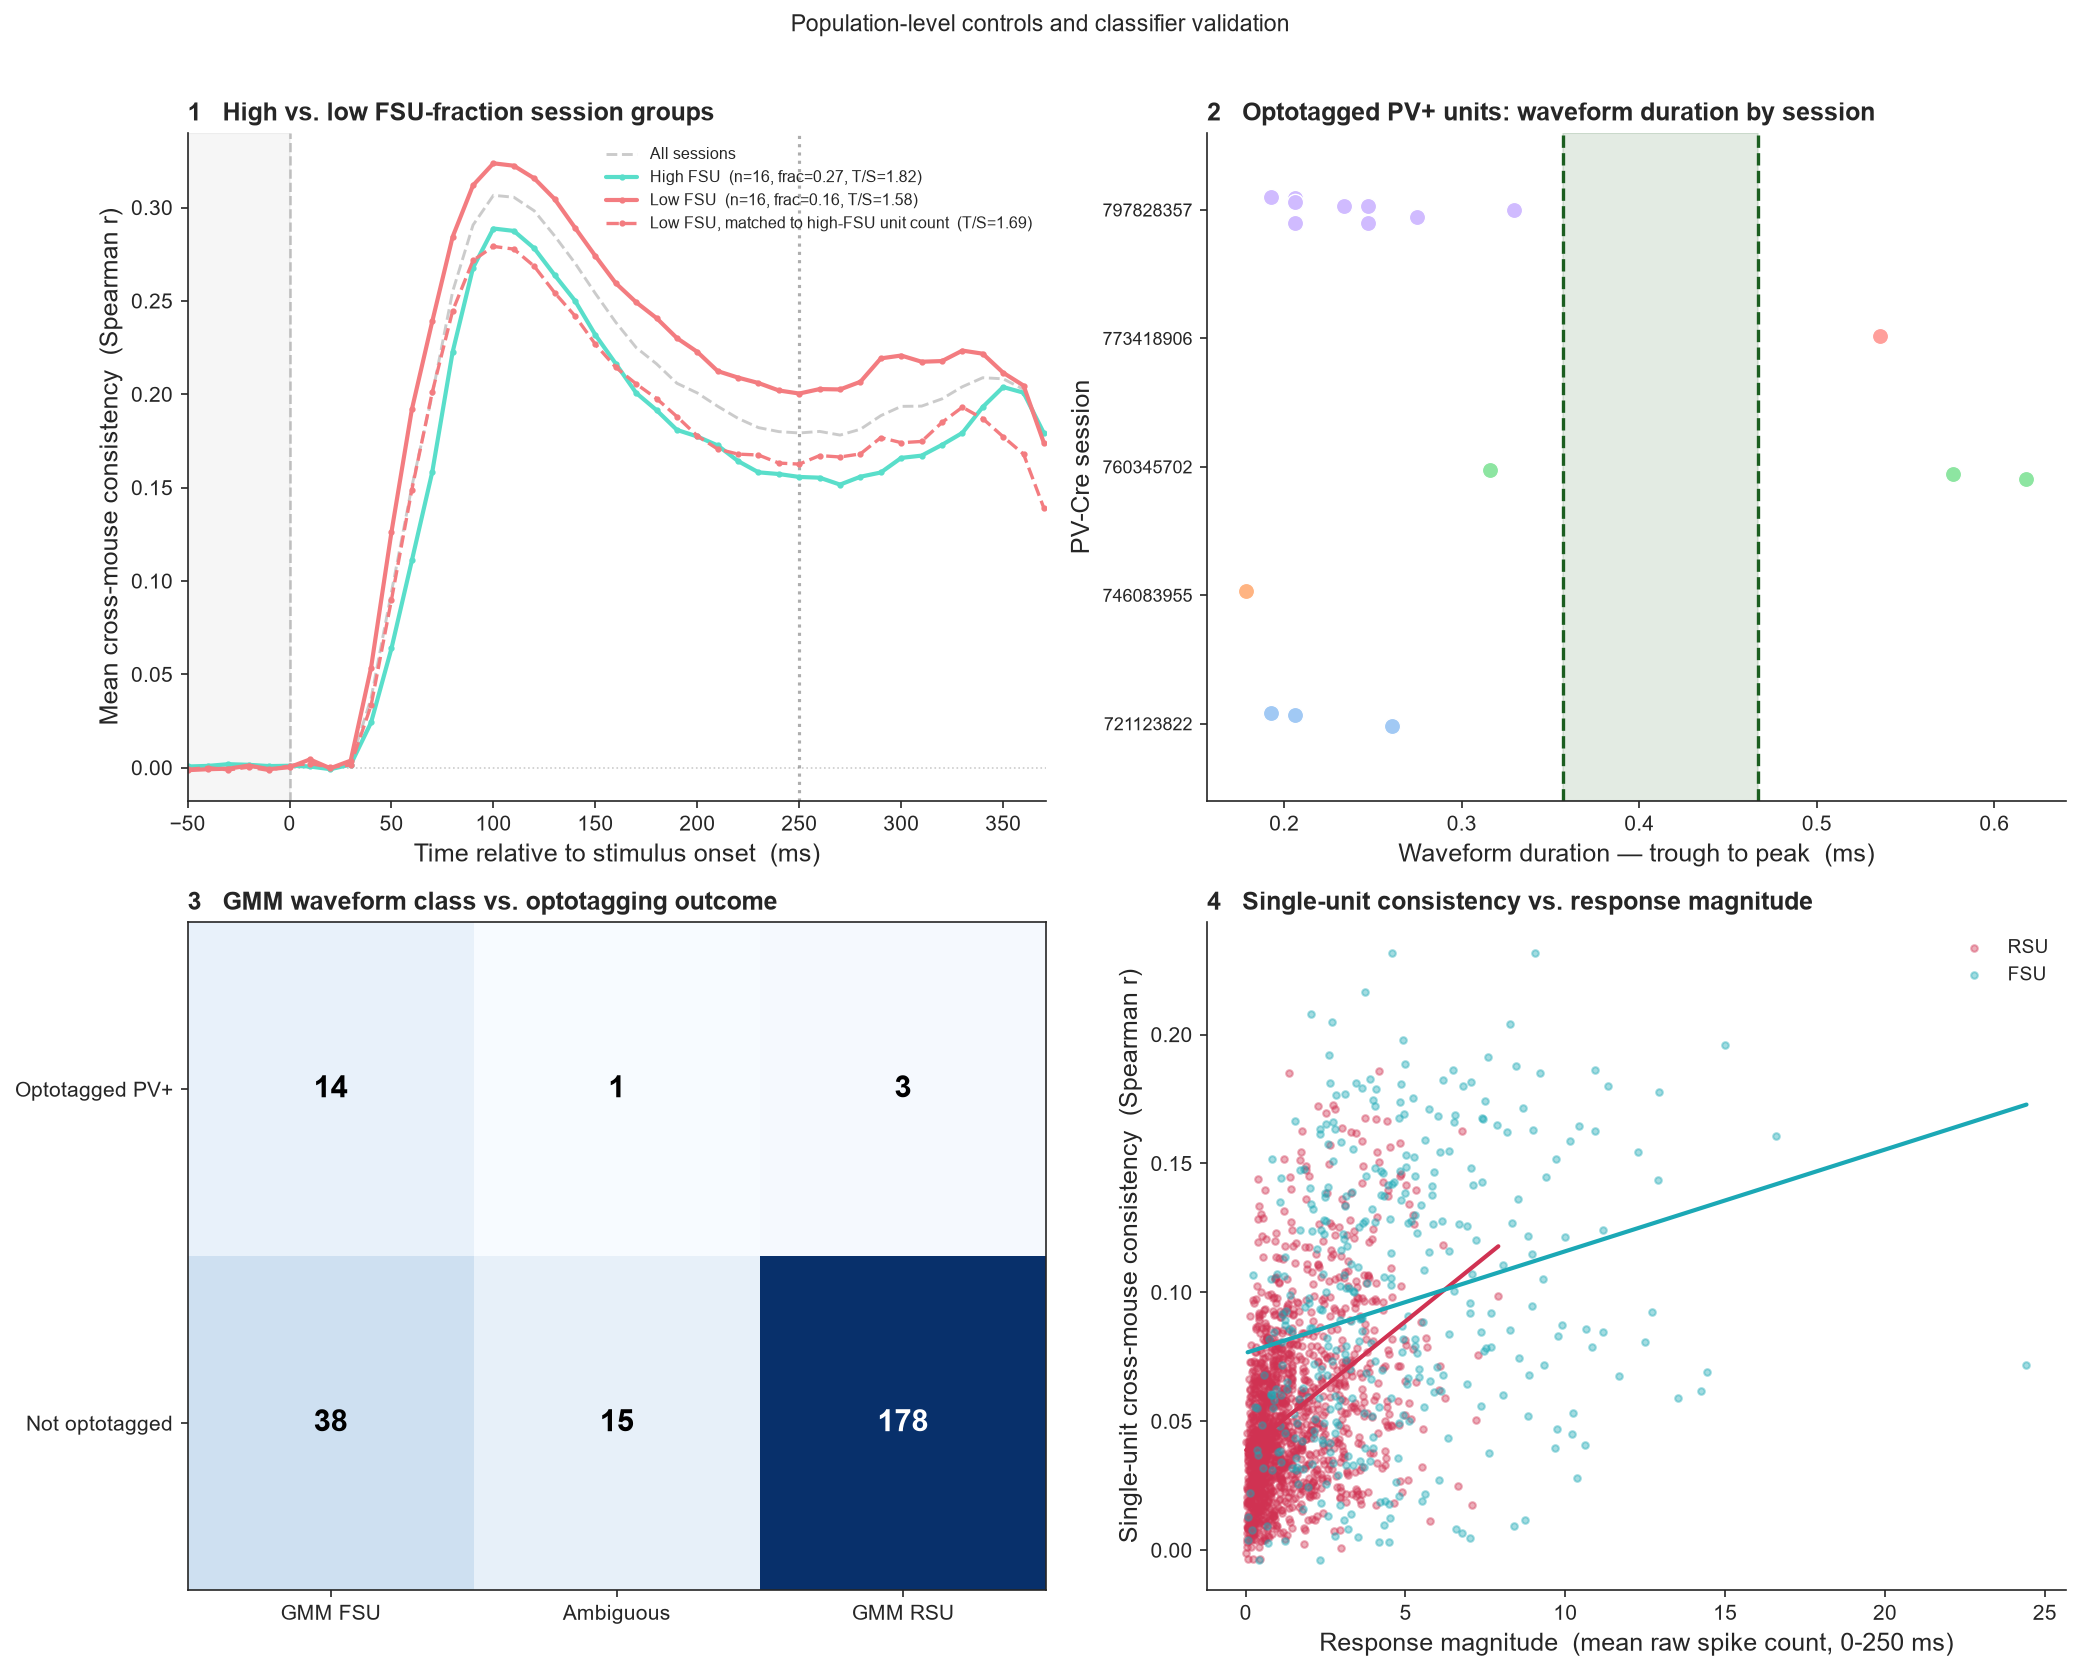
\includegraphics[width=\textwidth]{figures/figS4_population_controls_and_validation.png}
  \caption{\textbf{Population-level controls and classifier validation.}
  \textbf{(1)} Sliding-window curves for sessions split at the median FSU
  fraction: all sessions (dashed grey), high FSU ($n = 16$, mean fraction
  $= 0.273$, T/S $= 1.82\times$), low FSU ($n = 16$, mean fraction $=
  0.157$, T/S $= 1.58\times$), and low FSU subsampled to the high-FSU
  group's mean unit count (T/S $= 1.69\times$).
  \textbf{(2)} Strip plot of optotagged PV$^+$ unit waveform durations by
  PV-Cre session ($n = 5$ sessions, 18 optotagged units total). Shaded
  band and dashed lines: GMM narrow/broad boundaries (0.357~ms and
  0.467~ms).
  \textbf{(3)} Confusion matrix: optotagging outcome vs.\ GMM-inferred
  class. Sensitivity (PV$^+$ $\to$ GMM FSU) $= 78\%$; precision (GMM FSU
  $\to$ PV$^+$) $= 27\%$.
  \textbf{(4)} Single-unit cross-mouse consistency vs.\ raw response
  magnitude, by cell class (RSU pink, FSU teal), with per-class linear
  trends.}
  \label{fig:Spoplevel}
\end{figure}

\begin{figure}[htbp]
  \centering
  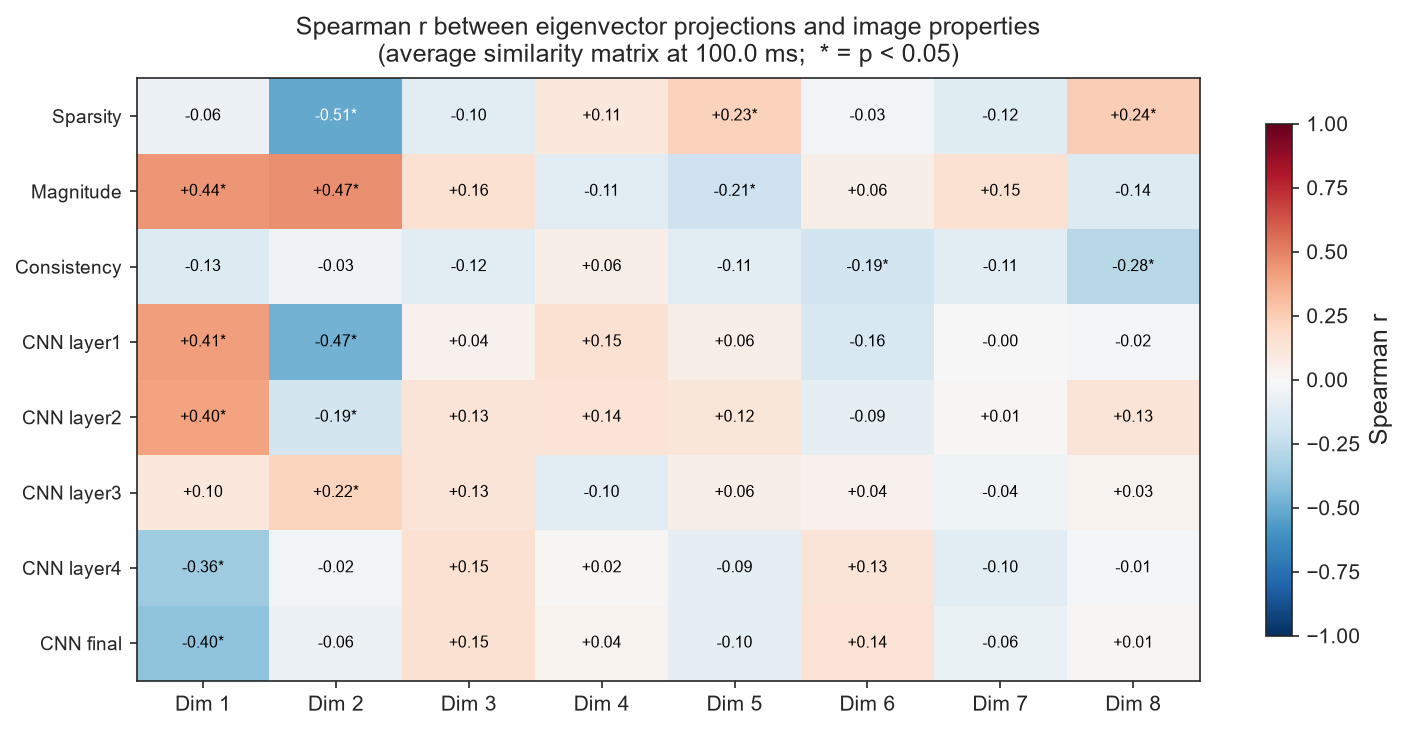
\includegraphics[width=\textwidth]{figures/figS5_eigenvec_properties.png}
  \caption{\textbf{Eigenvector loadings on image properties (full
  heatmap).}
  Spearman $r$ between eigenvector projections and image properties
  (sparsity, magnitude, consistency, CNN layers~1--4) for the top 8
  dimensions of the average cosine similarity matrix at 100~ms.
  Asterisks: $p < 0.05$. Dim~1 reflects signal strength and early CNN
  features; Dim~2 reflects sparsity and spatial scale.}
  \label{fig:Seigen}
\end{figure}

\begin{figure}[htbp]
  \centering
  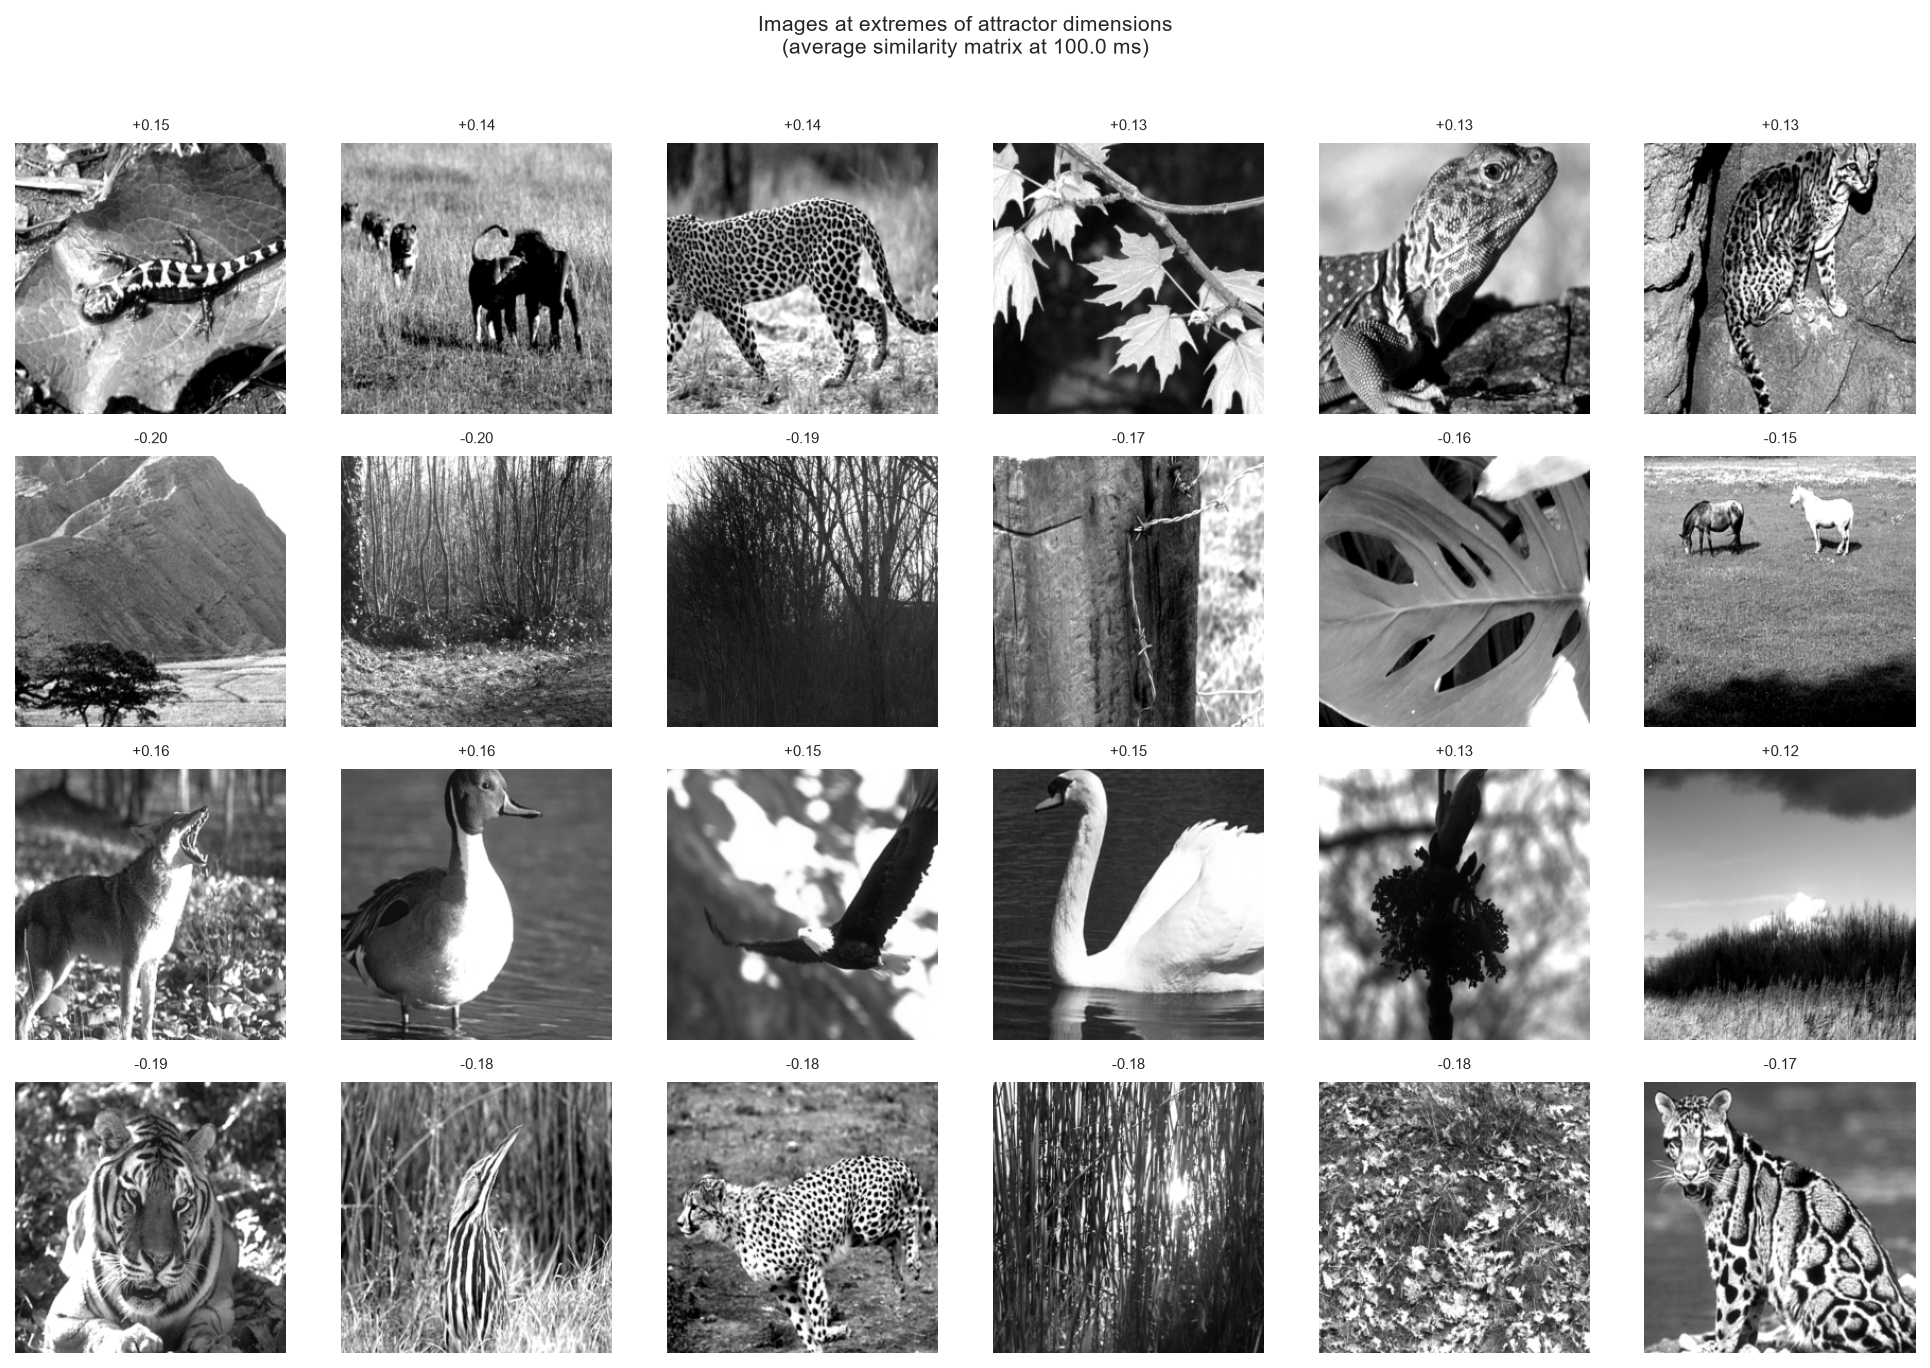
\includegraphics[width=\textwidth]{figures/figS6_attractor_gallery.png}
  \caption{\textbf{Attractor-space image gallery.}
  Images at the extremes of Dim~1 (signal-strength axis) and Dim~2
  (sparsity axis) of the average similarity matrix at 100~ms (top 6 and
  bottom 6 projections per dimension).}
  \label{fig:Sattractor}
\end{figure}

\begin{figure}[htbp]
  \centering
  
\includegraphics[width=\textwidth]{figures/figS7_rank_stability.png}
  \caption{\textbf{Image-ranking stability across the response epoch.}
  \textbf{(A)} Spearman rank-correlation matrix of per-image consistency
  across six epochs ($-25$, 25, 50, 100, 175, 250~ms). Image rankings are
  near-zero before 50~ms, correlated between peak and sustained epochs
  (100 vs.\ 250~ms: $r = 0.652$), and near-zero between pre-stimulus and
  any post-stimulus epoch.
  \textbf{(B)} Rolling Spearman correlation of per-image consistency at
  each sliding window vs.\ the 100~ms reference. Significance coding
  (filled marker: $p < 0.05$, hollow marker: n.s.) uses uncorrected
  $p$-values for illustration; overlapping windows are not independent.}
  \label{fig:Srank}
\end{figure}

\begin{figure}[htbp]
  \centering
  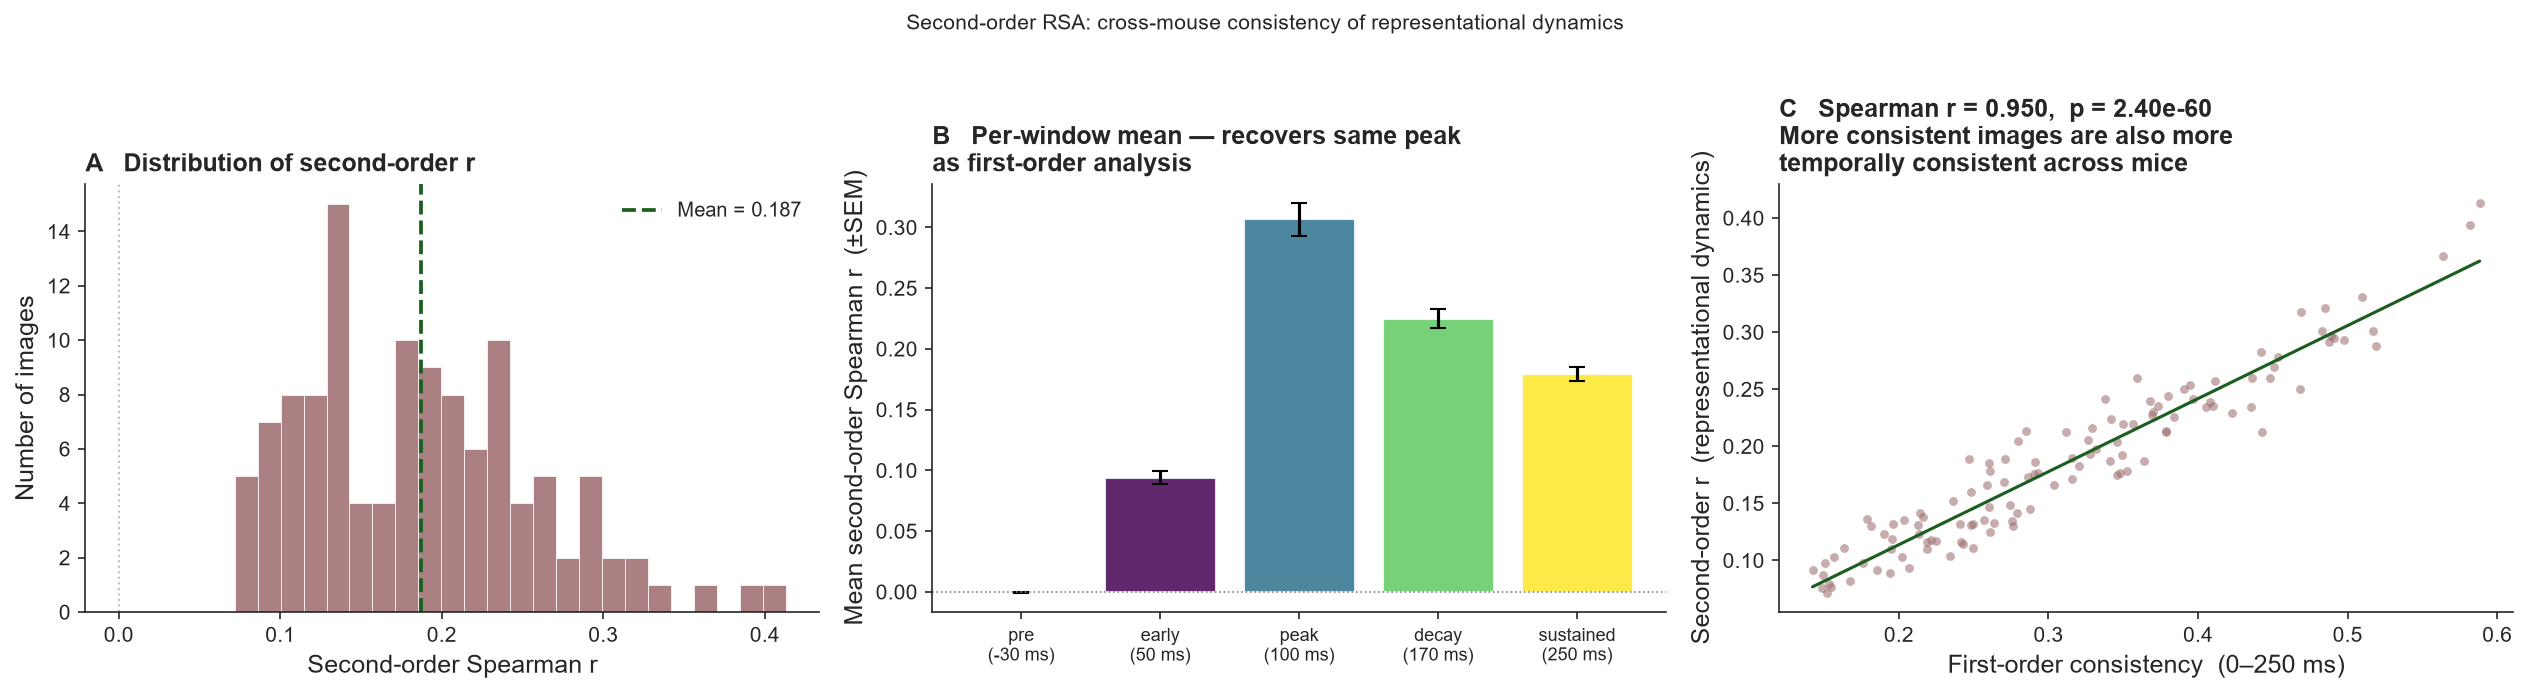
\includegraphics[width=\textwidth]{figures/figS8_second_order_rsa.png}
  \caption{\textbf{Second-order RSA recovers the same temporal peak.}
  \textbf{(A)} Distribution of second-order Spearman $r$ across 118 images
  (mean $= 0.187$; all images $> 0$).
  \textbf{(B)} Per-window mean second-order $r$ (bars $\pm$ SEM across
  images). The peak window (100~ms) yields the highest value
  ($r = 0.307$), matching the first-order consistency peak exactly.
  \textbf{(C)} Second-order $r$ vs.\ first-order consistency
  (Spearman $r = 0.950$, $p = 2.4 \times 10^{-60}$): the near-redundancy
  of the two measures indicates second-order RSA tracks the same
  underlying signal as first-order consistency, rather than providing an
  orthogonal confirmation of it.}
  \label{fig:Ssecondorder}
\end{figure}

\begin{figure}[htbp]
  \centering
  
\includegraphics[width=\textwidth]{figures/figS10_adaptation_control.png}
  \caption{\textbf{Adaptation control extended.}
  \textbf{(A)} Distribution of per-image (early $-$ late) consistency
  differences (mean $= +0.015$; one-sample $t$-test $p = 1.1 \times
  10^{-8}$). Positive mean indicates slight attenuation in the second
  half, opposite to a shared adaptation confound.
  \textbf{(B)} Early-half per-image consistency vs.\ full-session
  consistency ($r = 0.985$, $p = 2.6 \times 10^{-90}$).
  \textbf{(C)} Late-half per-image consistency vs.\ full-session
  consistency ($r = 0.984$, $p = 2.4 \times 10^{-88}$).}
  \label{fig:Sadapt}
\end{figure}

% ── References ────────────────────────────────────────────────────────────────
\clearpage
\bibliographystyle{plainnat}
\bibliography{references}

\end{document}